% =================================================================================================
% File:			capitolo_3.tex
% Description:	Definisce il capitolo che descrive generalmente il prodotto per il commitente
% Created:		2014-12-10
% Author:		Roetta Marco
% Email:		roetta.marco@mashup-unipd.it
% =============================================================================================================================
% Modification History:
% Version		Modifier Date		Change																			Author
% 0.0.1 		2014-12-30 			aggiunta sezione e iniziata stesura												Roetta Marco
% =============================================================================================================================
% 0.0.2 		2015-01-12 			Aggiunto elenco Casi d'uso incompleto											Roetta Marco
% =============================================================================================================================
% 0.0.3 		2015-01-12 			Aggiunta descrizione ai casi principali											Roetta Marco
% =============================================================================================================================
% 0.0.4 		2015-01-13 			Aggiunte altre descrizioni				 										Roetta Marco
% =============================================================================================================================
% 0.0.5 		2015-01-13 			Completato elenco UC					 										Roetta Marco
% =============================================================================================================================
% 0.0.6 		2015-01-15 			Modifica UC dopo incontro				 										Roetta Marco
% =============================================================================================================================
% 0.1.0 		2015-01-15 			Completata sezione						 										Roetta Marco
% =============================================================================================================================
% 0.1.1 		2015-01-15 			Correzioni ortografiche					 										Roetta Marco
% =============================================================================================================================
% 1.0.0 		2015-01-20 			Inizio Verifica				 													Nicola Faccin
% =============================================================================================================================
% 1.0.1 		2015-02-26 			Aggiunti UC2 e figli		 													Carnovalini Filippo
% =============================================================================================================================
% 2.0.1			2015-03-11			modificata descrizione UC1.3													Tesser Paolo
% =============================================================================================================================
% 2.0.2			2015-03-11			rimossi UC non pertinenti con la nuova analisi, UC1.3.2/3/4/5 con deriviati		Tesser Paolo
% =============================================================================================================================
% 2.0.3			2015-03-11			modificati UC riguardanti i servizi REST										Tesser Paolo
% =============================================================================================================================
% 2.0.4			2015-03-12			modificato UC1.3 e aggiunti derivati UC1.3.1 e UC1.3.2							Tesser Paolo
% =============================================================================================================================
% 2.0.5			2015-03-13			aggiunto UC2.4 e sistemato UC2													Tesser Paolo
% =============================================================================================================================
% 2.0.6			2015-03-14			aggiunto UC1.3.1.1/2/3/4


% CONTENUTO DEL CAPITOLO

\section{Casi d'uso}

\subsection{UC1: Caso d'uso pubblico}
\begin{figure}[!htbp]
	\centering
	\centerline{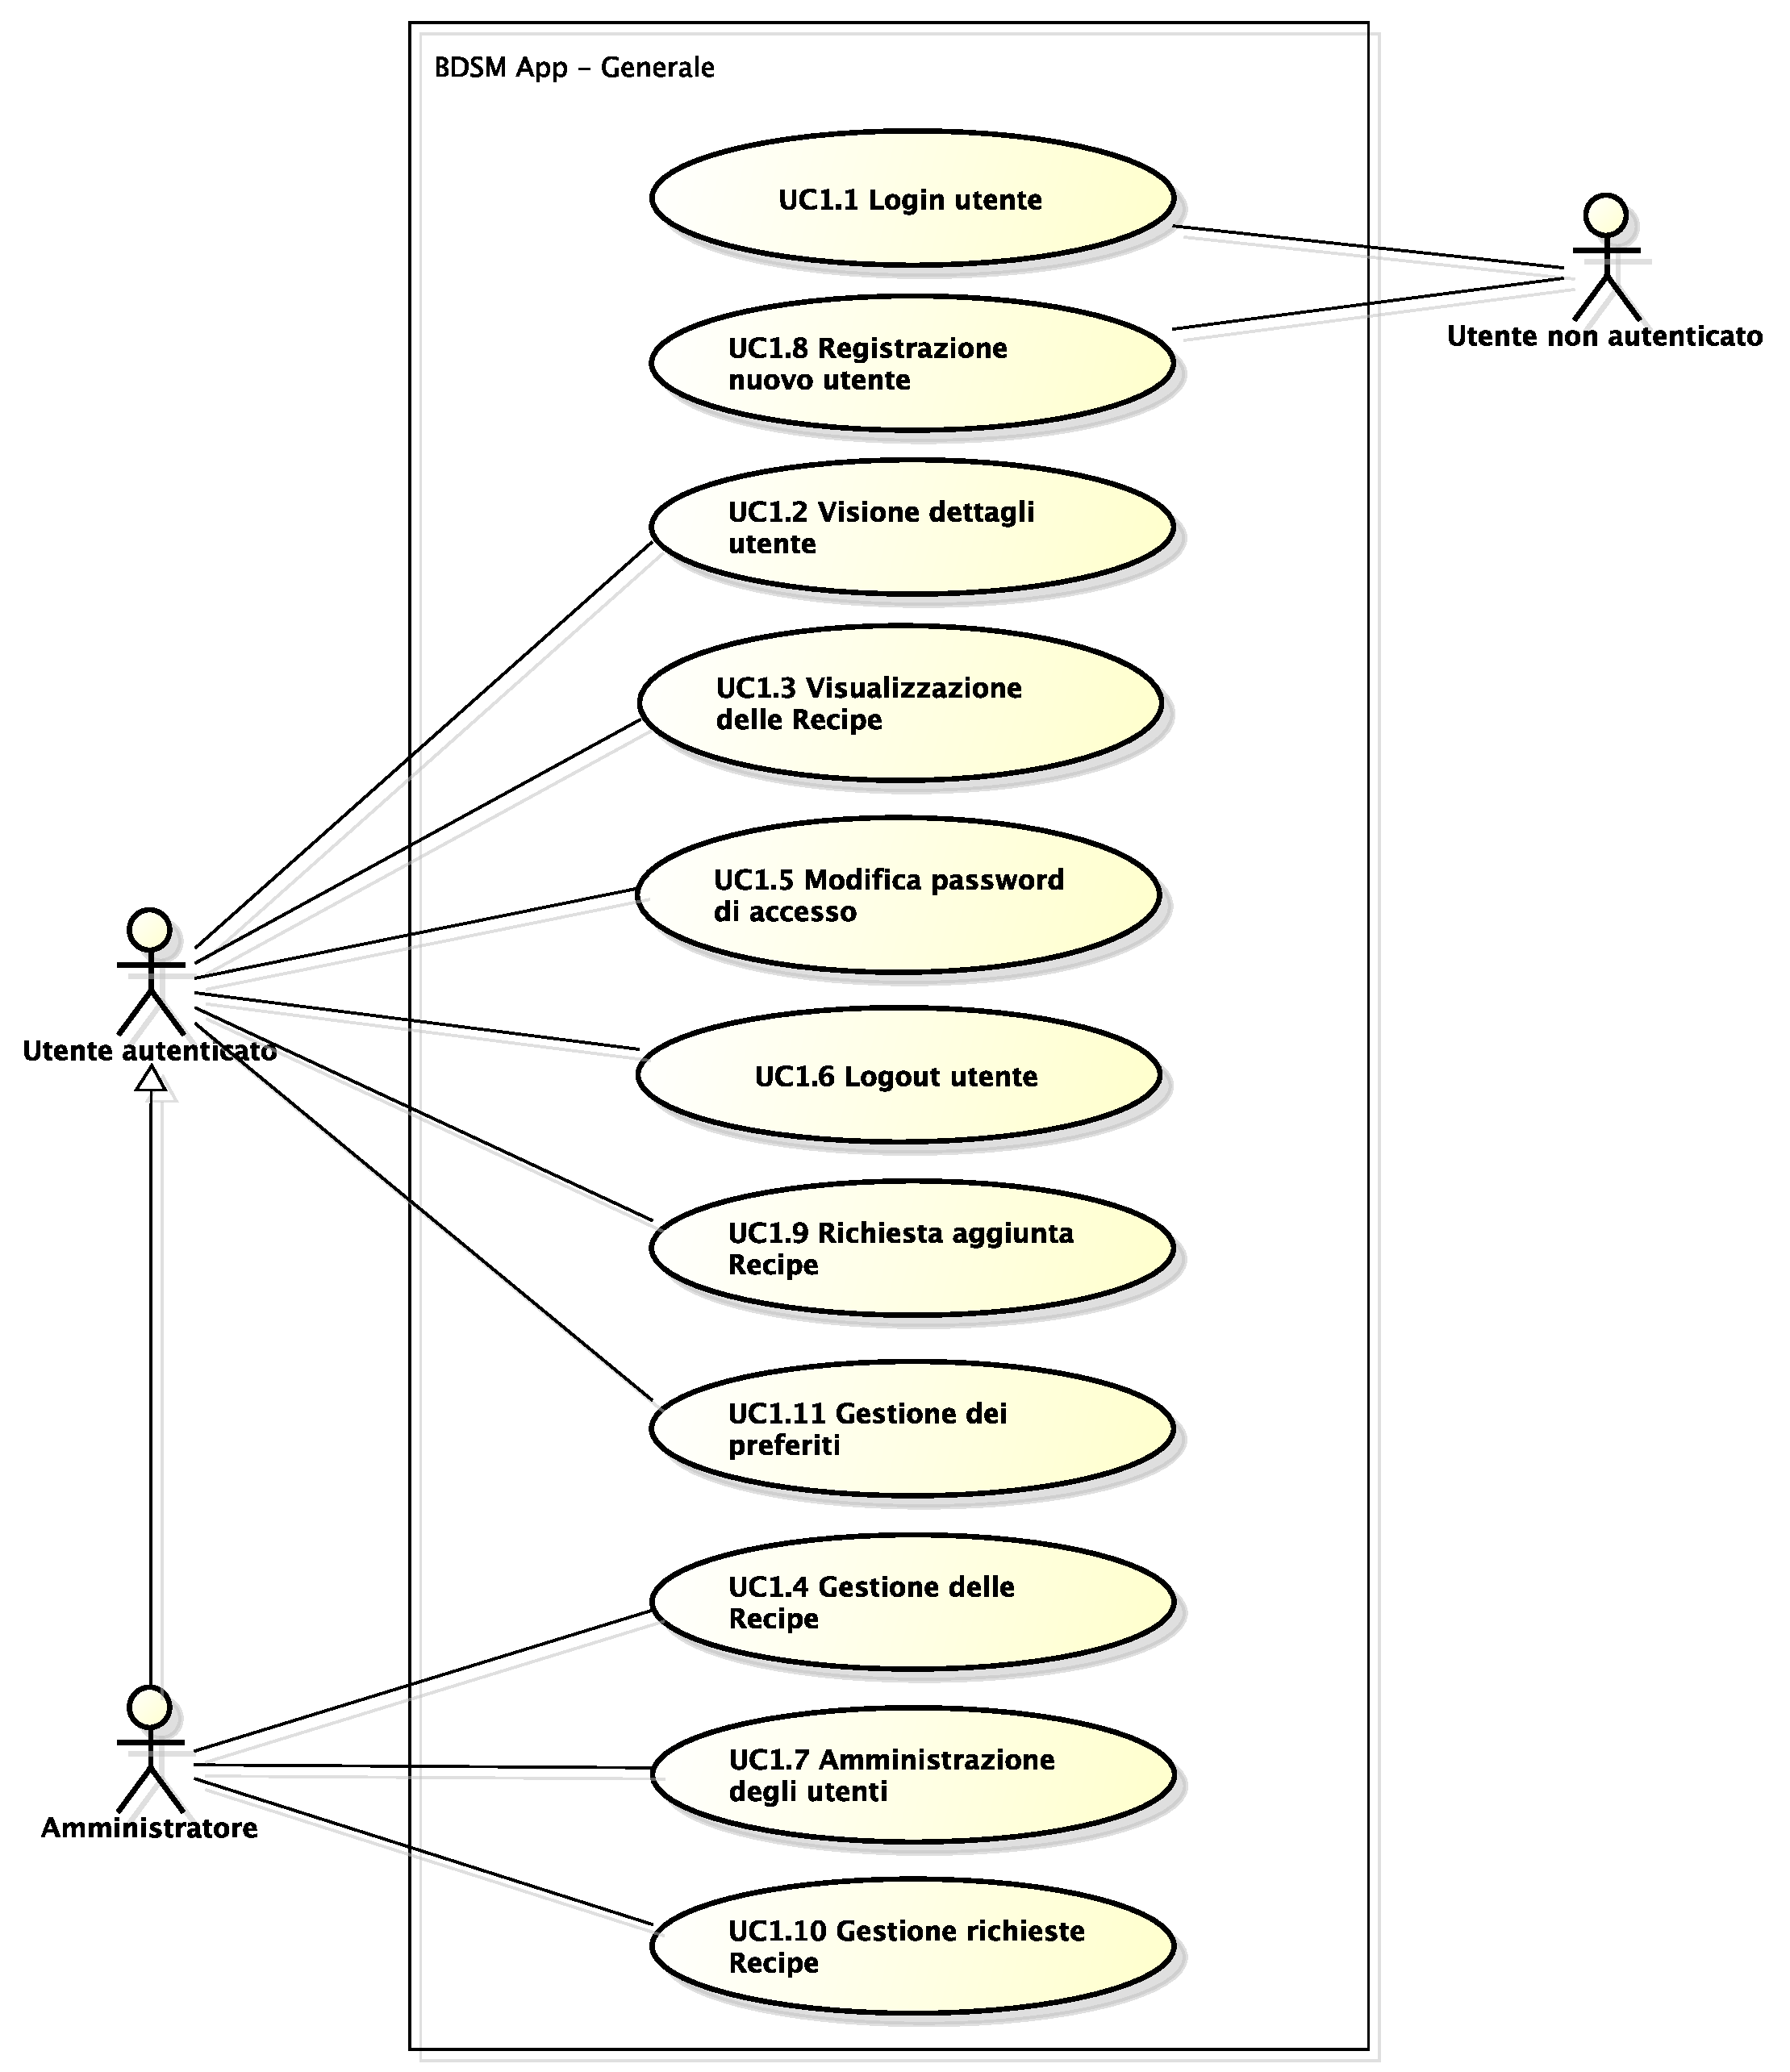
\includegraphics[scale=0.45]{./images/UC1.pdf}}
	\caption{UC1 - Caso d'uso pubblico}
\end{figure}

\begin{itemize}
	\item \textbf{Attori:}
	\begin{itemize}
		\item utente non autenticato: utente non ancora noto al sistema che accede al servizio;
		\item utente autenticato: utente autenticato che ha accesso al servizio;
		\item utente amministratore: utente autenticato che ha accesso al servizio e dispone dei permessi per visualizzare tutte le aree;
	\end{itemize}
	\item \textbf{Descrizione:} dopo l'accesso al servizio:
	\begin{itemize}
		\item un utente sconosciuto può autenticarsi, o se è al primo accesso al servizio può registrarsi per ottenere delle credenziali valide;
		\item un utente autenticato può vedere statistiche, modificare la propria password, visualizzare, creare e modificare le proprie View;
		\item un utente amministratore può fare tutte le operazioni di un utente autenticato, più ha la possibilità di eliminare un utente e tutte le sue View e modificarne i privilegi;
	\end{itemize}
	\item \textbf{Precondizione:} l'utente autenticato, l'utente non autenticato o l'amministratore hanno caricato la prima pagina del servizio;
	Viene visualizzato un messaggio di errore nel caso le informazioni di accesso inserite siano errate;
	\item \textbf{Flusso principale degli eventi:}
	\begin{enumerate}
		\item Login utente (UC1.1);
		\item Visualizza informazione utente e statistiche (UC1.2);
		\item Visualizzazione delle Recipe (UC1.3);
		\item Richiesta aggiunta Recipe (UC1.9);
		\item Gestione dei preferiti (UC1.11);
		\item Gestione delle Recipe (UC1.4);
		\item Modifica password di accesso (UC1.5);
		\item Logout utente (UC1.6);
		\item Amministrazione utenti (UC1.7);
		\item Registrazione nuovo utente (UC1.8);
		\item Visione richieste utente (UC1.10).
	\end{enumerate}
	\item \textbf{Postcondizione:} il servizio ha erogato correttamente le funzionalità richieste dall'utente;
\end{itemize}
% FINE USE CASE %

\pagebreak


\subsection{UC1.1: Login utente}

\begin{figure}[htbp]
	\centering
	\centerline{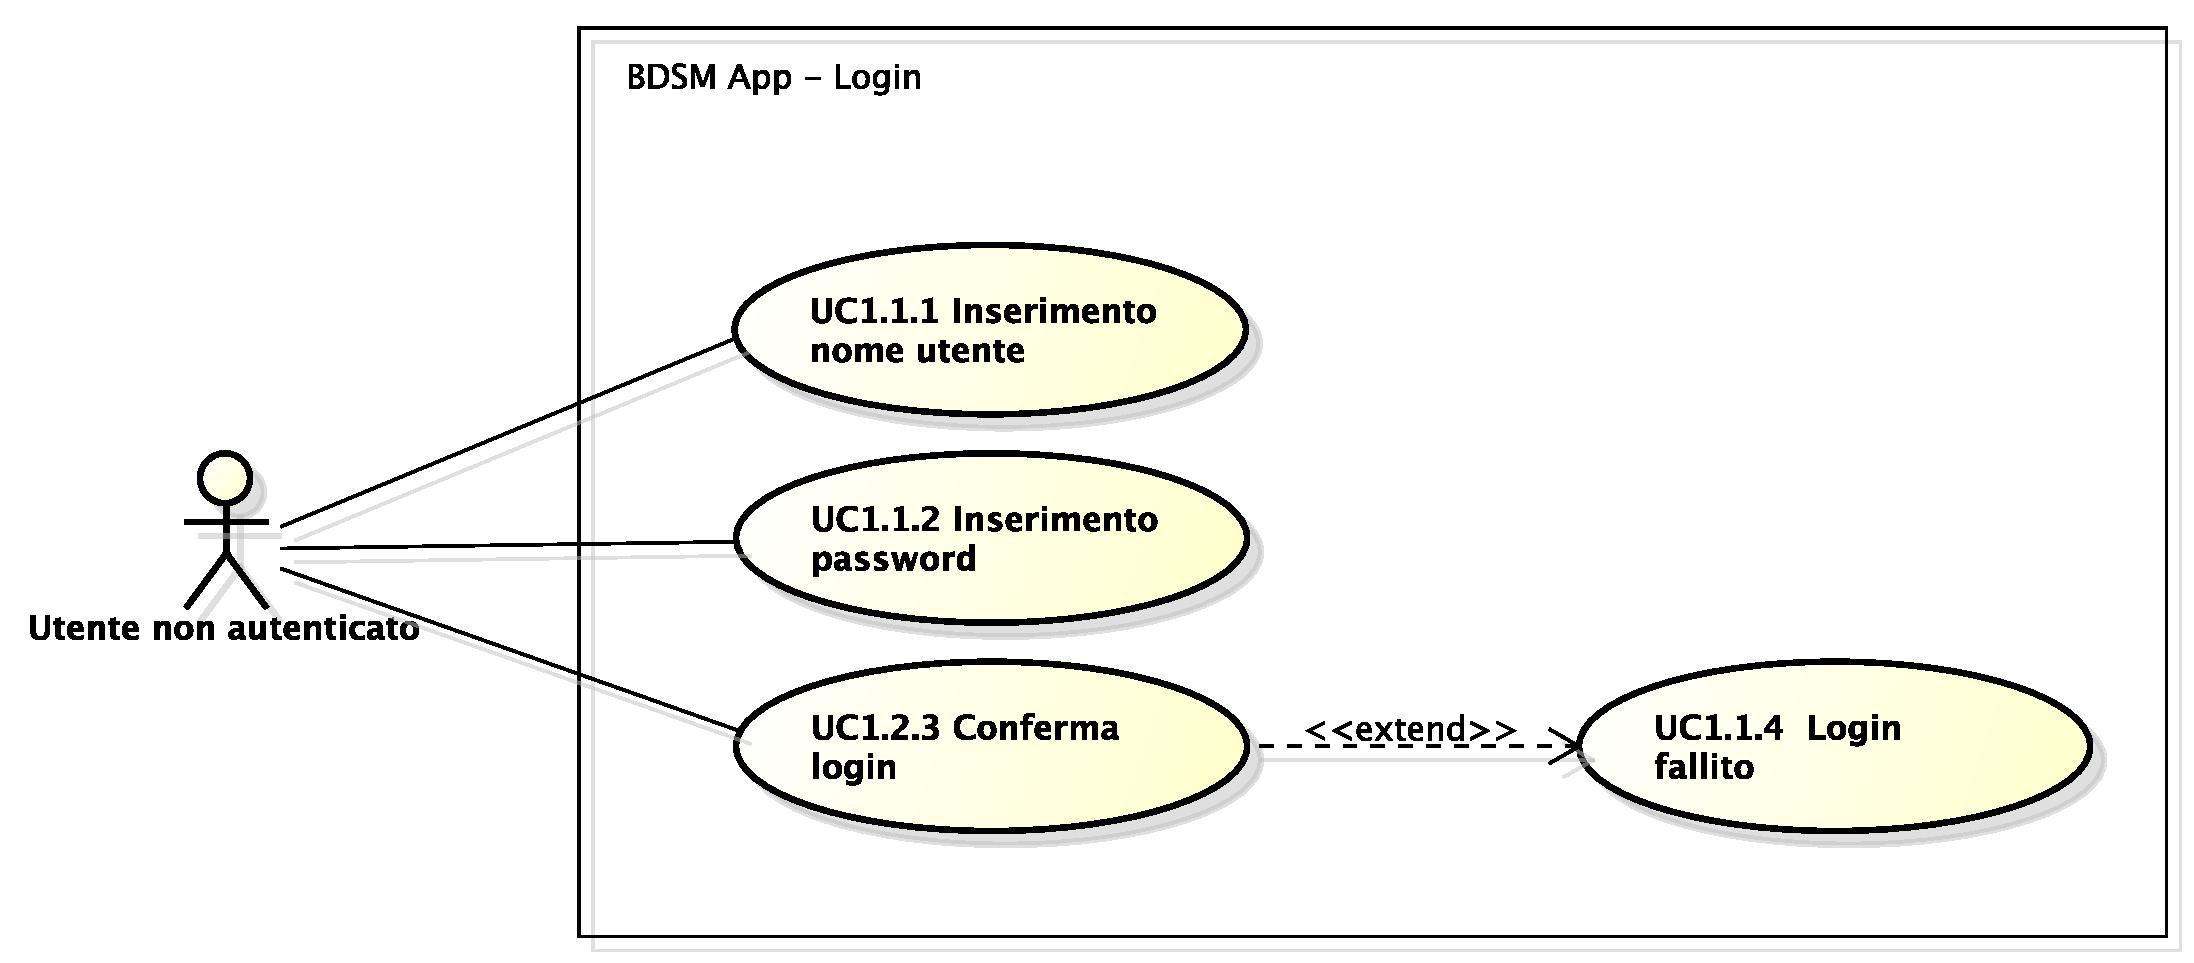
\includegraphics[scale=0.45]{./images/UC1_1.pdf}}
	\caption{UC1.1 - Login utente}
\end{figure}

\begin{itemize}
	\item \textbf{Attori:}
	\begin{itemize}
		\item utente non autenticato: utente non ancora noto al sistema che accede al servizio;
	\end{itemize}
	\item \textbf{Descrizione:} l'utente può autenticarsi per poter accedere ai servizi offerti dalla piattaforma utilizzando la schermata di login;
	\item \textbf{Precondizione:} l'utente che accede alla pagina di accesso è sconosciuto al sistema;
	\item \textbf{Flusso principale degli eventi:}
	\begin{enumerate}
		\item Inserimento username (UC1.1.1);
		\item Inserimento password (UC1.1.2);
		\item Conferma login (UC1.1.3);
	\end{enumerate}
	\item \textbf{Postcondizione:} l'utente è riconosciuto dal sistema;
	\item \textbf{Estensioni:} Login fallita (UC1.1.4).
\end{itemize}
% FINE USE CASE %

\subsubsection{UC1.1.1: Inserimento username}
\begin{itemize}
	\item \textbf{Attori:}
	\begin{itemize}
		\item utente non autenticato: utente non ancora noto al sistema che accede al servizio;
	\end{itemize}
	\item \textbf{Descrizione:} l'utente non autenticato deve poter inserire l'username ai fini dell'autenticazione;
	\item \textbf{Precondizione:} il sistema fornisce una schermata in cui è possibile inserire l’username;
	\item \textbf{Scenario principale:} l'utente non autenticato inserisce l'username nell'apposito campo.
	\item \textbf{Postcondizione:} il sistema ha l'informazione relativa all'username.

\end{itemize}
% FINE USE CASE %

\subsubsection{UC1.1.2: Inserimento password}
\begin{itemize}
	\item \textbf{Attori:}
	\begin{itemize}
		\item utente non autenticato: utente non ancora noto al sistema che accede al servizio;
	\end{itemize}
	\item \textbf{Descrizione:} l'utente non autenticato deve poter inserire la propria password ai fini dell'autenticazione;
	\item \textbf{Precondizione:} il sistema fornisce una schermata in cui è possibile inserire la password;
	\item \textbf{Scenario principale:} l'utente non autenticato inserisce la password nell'apposito campo;
	\item \textbf{Postcondizione:} il sistema ha l'informazione relativa alla password inserita dall'utente.
\end{itemize}
% FINE USE CASE %

\subsubsection{UC1.1.3: Conferma login}
\begin{itemize}
	\item \textbf{Attori:}
	\begin{itemize}
		\item utente non autenticato: utente non ancora noto al sistema che accede al servizio;
	\end{itemize}
	\item \textbf{Descrizione:} viene richiesto all'utente di confermare i dati inseriti con la pressione di un pulsante di conferma in modo da avviare il processo di autenticazione;
	\item \textbf{Precondizione:} il sistema fornisce un pulsante per confermare il login;
	\item \textbf{Scenario principale:} l'utente non autenticato preme l'apposito pulsante per confermare i dati inseriti;
	\item \textbf{Postcondizione:} l'utente ha eseguito il login.
\end{itemize}

\subsubsection{UC1.1.4: Login fallita}
\begin{itemize}
	\item \textbf{Attori:}
	\begin{itemize}
		\item utente non autenticato: utente non ancora noto al sistema che accede al servizio;
	\end{itemize}
	\item \textbf{Descrizione:} viene mostrato all'utente un messaggio di errore che riporta la non correttezza dei dati inseriti;
	\item \textbf{Precondizione:} il sistema ha ricevuto una richiesta di accesso da uno username errato o una password non associata allo username esistente indicato.
	\item \textbf{Scenario principale:} l'utente non autenticato visualizza il messaggio di errore;
	\item \textbf{Postcondizione:} l'utente ha preso atto del messaggio di errore.
\end{itemize}
% FINE USE CASE %

\pagebreak


\subsection{UC1.2: Visione dettagli utente}
\begin{figure}[htbp]
	\centering
	\centerline{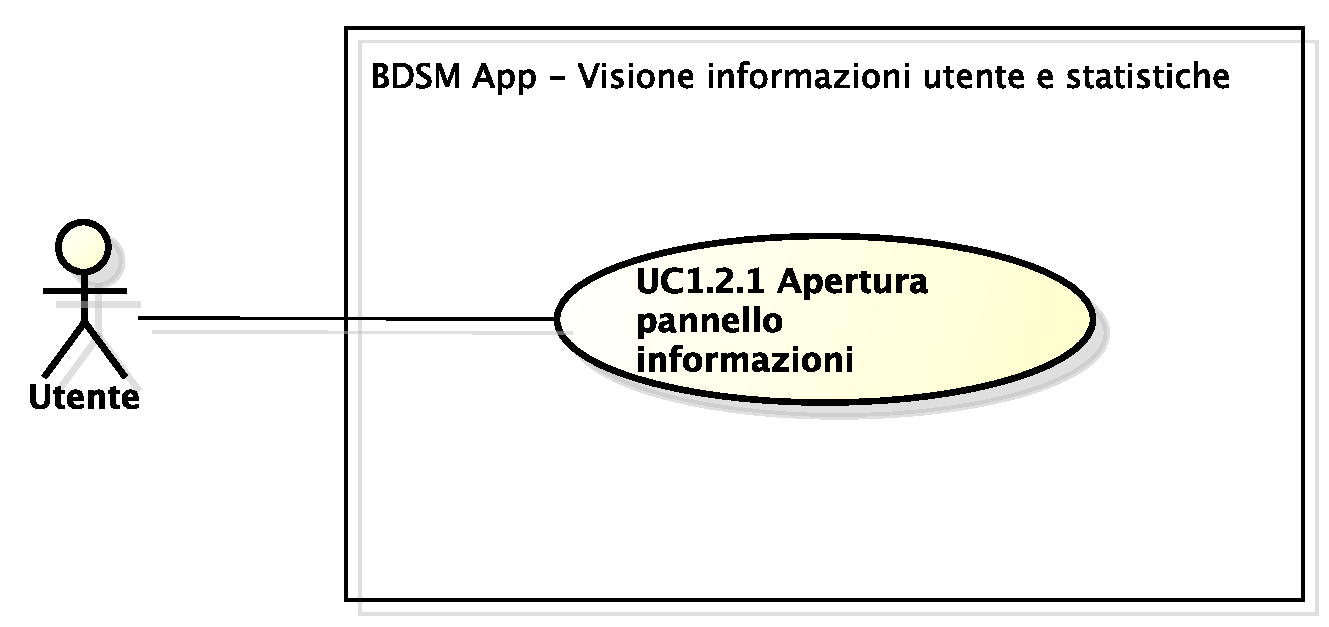
\includegraphics[scale=0.45]{./images/UC1_2.pdf}}
	\caption{UC1.2 - Visione dettagli utente}
\end{figure}

\begin{itemize}
	\item \textbf{Attori:}
	\begin{itemize}
		\item utente autenticato: utente autenticato che ha accesso al servizio;
	\end{itemize}
	\item \textbf{Descrizione:} gli utenti autenticati possono vedere una serie di informazioni relative alla 	loro attività, come la data dell'ultimo accesso effettuato e il numero di ricette e viste attive;
	\item \textbf{Precondizione:} l'utente deve essere autenticato;
	\item \textbf{Flusso principale degli eventi:}
	\begin{enumerate}
		\item Visualizza informazioni utente (UC1.2.1);
		\item Visualizza statistiche utente (UC1.2.2).
	\end{enumerate}
	\item \textbf{Postcondizione:} le informazioni richieste dall'utente sono state fornite;
\end{itemize}
% FINE USE CASE %

\subsubsection{UC1.2.1: Visualizza informazioni utente}
\begin{itemize}
	\item \textbf{Attori:}
	\begin{itemize}
		\item utente autenticato: utente autenticato che ha accesso al servizio;
	\end{itemize}
	\item \textbf{Descrizione:} selezionando il pulsante dettagli utente viene mostrata all'utente una pagina con il riepilogo dei sui dati, quali:
	\begin{itemize}
		\item il nome utente;
		\item l'indirizzo email associato;
		\item la data dell'ultimo accesso effettuato;
	\end{itemize}
	\item \textbf{Precondizione:} l'utente ha selezionato il pulsante per l'accesso ai dettagli utente;
	\item \textbf{Flusso principale degli eventi:}
	\begin{enumerate}
    \item Visualizza username (UC1.2.1.1);
    \item Visualizza email (UC1.2.1.2);
    \item Visualizza ultimo accesso (UC1.2.1.3).
  \end{enumerate}
	\item \textbf{Postcondizione:} l'utente ha ottenuto le informazioni richieste;
\end{itemize}
% FINE USE CASE %

\subsubsection{UC1.2.1.1: Visualizza username}
\begin{itemize}
	\item \textbf{Attori:}
	\begin{itemize}
		\item utente autenticato: utente autenticato che ha accesso al servizio;
	\end{itemize}
	\item \textbf{Descrizione:} nella sezione delle informazioni personali l'utente può visualizzare il suo username;
	\item \textbf{Precondizione:} l'utente ha effettuato l'accesso alla pagina di dettaglio dei dati personali;
	\item \textbf{Scenario principale:} l'utente visualizza il proprio username;
	\item \textbf{Postcondizione:} l'utente ha visualizzato il suo username.
\end{itemize}
% FINE USE CASE %

\subsubsection{UC1.2.1.2: Visualizza indirizzo email}
\begin{itemize}
	\item \textbf{Attori:}
	\begin{itemize}
		\item utente autenticato: utente autenticato che ha accesso al servizio;
	\end{itemize}
	\item \textbf{Descrizione:} nella sezione delle informazioni personali l'utente può visualizzare il suo indirizzo email;
	\item \textbf{Precondizione:} l'utente ha effettuato l'accesso alla pagina di dettaglio dei dati personali;
	\item \textbf{Scenario principale:} l'utente visualizza il proprio indirizzo email;
	\item \textbf{Postcondizione:} l'utente ha visualizzato il suo indirizzo email.
\end{itemize}
% FINE USE CASE %

\subsubsection{UC1.2.1.3: Visualizza ultimo accesso}
\begin{itemize}
	\item \textbf{Attori:}
	\begin{itemize}
		\item utente autenticato: utente autenticato che ha accesso al servizio;
	\end{itemize}
	\item \textbf{Descrizione:} nella sezione delle informazioni personali l'utente può visualizzare data ed ora del suo ultimo accesso;
	\item \textbf{Precondizione:} l'utente ha effettuato l'accesso alla pagina di dettaglio dei dati personali;
	\item \textbf{Scenario principale:} l'utente visualizza i dettagli del suo ultimo accesso;
	\item \textbf{Postcondizione:} l'utente ha visualizzato i dettagli del suo ultimo accesso.
\end{itemize}
% FINE USE CASE %

\subsubsection{UC1.2.2: Visualizza statistiche utente}
\begin{itemize}
	\item \textbf{Attori:}
	\begin{itemize}
		\item utente autenticato: utente autenticato che ha accesso al servizio;
	\end{itemize}
	\item \textbf{Descrizione:} selezionando il pulsante dettagli utente viene mostrata all'utente una pagina con il riepilogo delle sue statistiche, quali:
	\begin{itemize}
		\item numero di View presenti fornite dal sistema;
		\item numero di Recipe fornite dal sistema;
	\end{itemize}
  \item \textbf{Precondizione:} l'utente ha selezionato il pulsante per l'accesso ai dettagli utente
	\item \textbf{Flusso principale degli eventi:}
	\begin{enumerate}
		\item Visualizza numero View attive (UC1.2.2.1)
		\item Visualizza numero Recipe disponibili (UC1.2.2.2)
	\end{enumerate}
	\item \textbf{Postcondizione:} l'utente ha ottenuto le informazioni richieste.
\end{itemize}
% FINE USE CASE %

\subsubsection{UC1.2.2.1: Visualizza numero View attive}
\begin{itemize}
	\item \textbf{Attori:}
	\begin{itemize}
		\item utente autenticato: utente autenticato che ha accesso al servizio;
	\end{itemize}
	\item \textbf{Descrizione:} nella sezione delle statistiche personali l'utente può visualizzare il numero di View attive;
	\item \textbf{Precondizione:} l'utente ha effettuato l'accesso alla pagina di dettaglio dei dati personali;
	\item \textbf{Scenario principale:} l'utente visualizza il numero di View attive;
	\item \textbf{Postcondizione:} l'utente ha visualizzato il numero di View attive.
\end{itemize}
% FINE USE CASE %

\subsubsection{UC1.2.2.2: Visualizza numero Recipe disponibili}
\begin{itemize}
	\item \textbf{Attori:}
	\begin{itemize}
		\item utente autenticato: utente autenticato che ha accesso al servizio;
	\end{itemize}
	\item \textbf{Descrizione:} nella sezione delle statistiche personali l'utente può visualizzare il numero di Recipe attualmente disponibili nel sistema;
	\item \textbf{Precondizione:} l'utente ha effettuato l'accesso alla pagina di dettaglio dei dati personali;
	\item \textbf{Scenario principale:} l'utente visualizza il numero di Recipe disponibili;
	\item \textbf{Postcondizione:} l'utente ha visualizzato il numero di Recipe disponibili.
\end{itemize}
% FINE USE CASE %

\pagebreak
\subsection{UC1.3: Visualizzazione delle Recipe}
\begin{figure}[!htbp]
	\centering
	\centerline{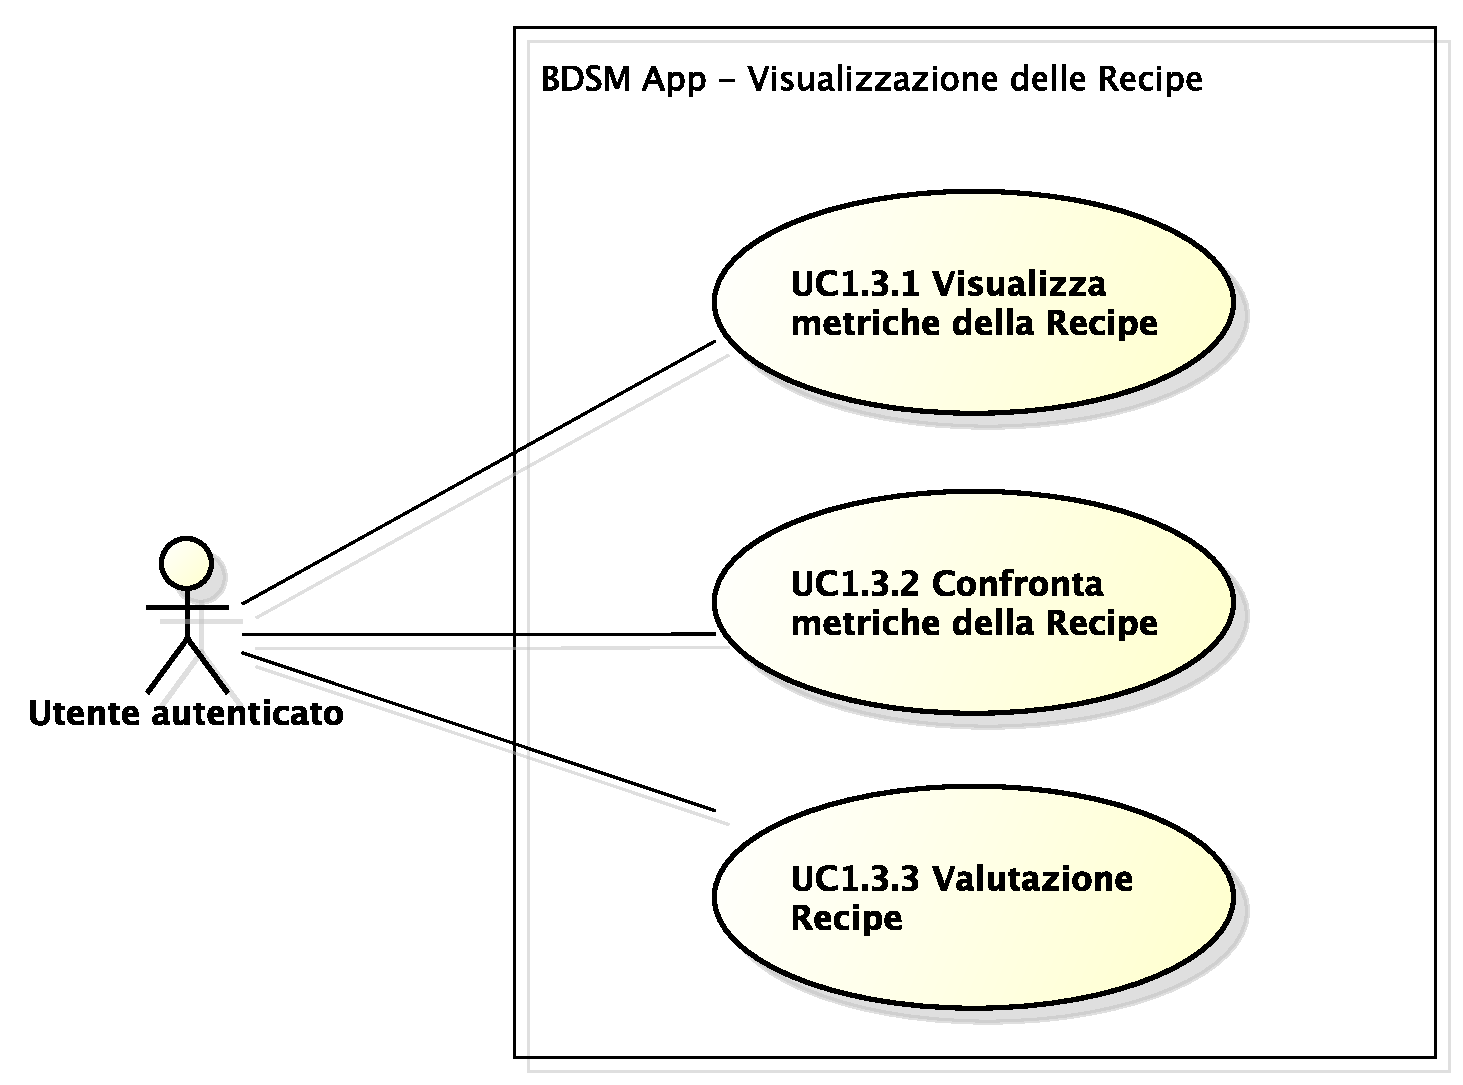
\includegraphics[scale=0.45]{./images/UC1_3.pdf}}
	\caption{UC1.3 - Visualizzazione delle Recipe}
\end{figure}

\begin{itemize}
	\item \textbf{Attori:}
	\begin{itemize}
		\item utente autenticato: utente autenticato che ha accesso al servizio;
	\end{itemize}
	\item \textbf{Descrizione:} gli utenti possono vedere in questa pagina le Recipe offerte dal sistema. Per ciascuna Recipe l'utente può decidere di visualizzare tutte le View associate o effettuare un confronto tra le View di quella Recipe.
	\item \textbf{Precondizione:} l'utente deve aver effettuato l'accesso nell'apposita pagina;
	\item \textbf{Flusso principale degli eventi:}
	\begin{enumerate}
		\item Visualizza metriche della Recipe (UC1.3.1);
		\item Confronta metriche della Recipe (UC1.3.2).
	\end{enumerate}
	\item \textbf{Postcondizione:} è stato fornito un elenco delle Recipe disponibili.
\end{itemize}
% FINE USE CASE %

\subsubsection{UC1.3.1: Visualizza metriche della Recipe}
\begin{figure}[!htbp]
	\centering
	\centerline{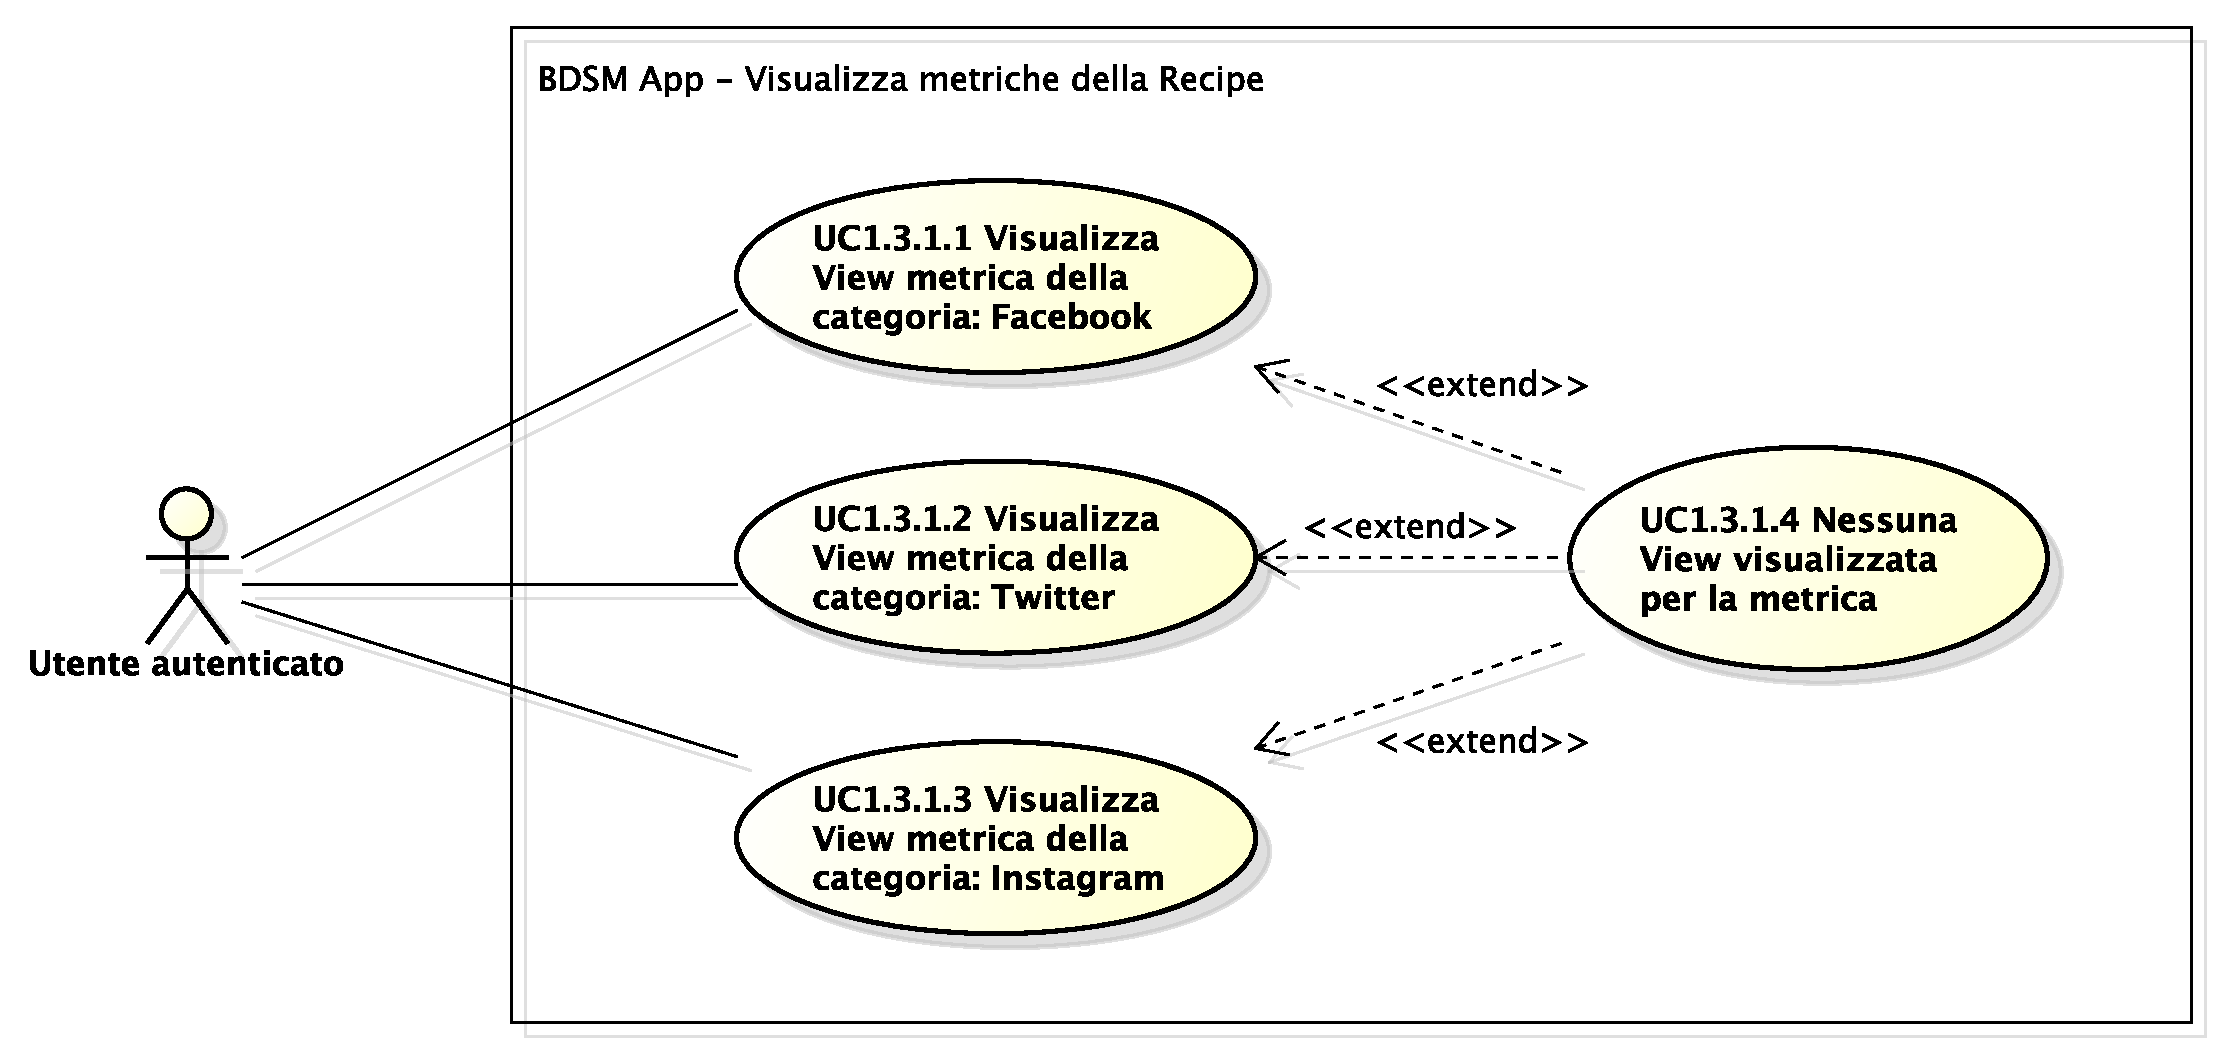
\includegraphics[scale=0.45]{./images/UC1_3_1.pdf}}
	\caption{UC1.3.1 - Visualizza metriche della Recipe}
\end{figure}

\begin{itemize}
	\item \textbf{Attori:}
	\begin{itemize}
		\item utente autenticato: utente autenticato che ha accesso al servizio;
	\end{itemize}
	\item \textbf{Descrizione:} l'utente visualizza un elenco di metriche che sono state scelte durante la creazione della Recipe (UC1.4.2). Ad ogni metrica sono associate le relative View offerte dal sistema. Le metriche vengono mostrate divise in base alla categoria di cui fanno parte. (es. Facebook, Twitter, Instagram, ...). Per ogni voce mostrata andrà fornito il nome, una descrizione e un pulsante per entrare nella visualizzazione delle View;
	\item \textbf{Precondizione:} l'utente è entrato nella visualizzazione di tutte le metriche della Recipe selezionata;
	\item \textbf{Flusso principale degli eventi:}
	\begin{enumerate}
		\item Visualizza View metrica della categoria: Facebook (UC1.3.1.1);
		\item Visualizza View metrica della categoria: Twitter (UC1.3.1.2);
		\item Visualizza View metrica della categoria: Instagram (UC1.3.1.3);
	\end{enumerate}
	\item \textbf{Postcondizione:} l'utente ha visualizzato tutte le metriche presenti nella Recipe a seconda della categoria scelta;
	\item \textbf{Estensioni:} Nessuna View visualizzata per la metrica (UC1.3.1.4).
\end{itemize}
% FINE USE CASE %

\subsubsection{UC1.3.1.1: Visualizza View metrica della categoria: Facebook}
\begin{itemize}
	\item \textbf{Attori:}
	\begin{itemize}
		\item utente autenticato: utente autenticato che ha accesso al servizio;
	\end{itemize}
	\item \textbf{Descrizione:} premendo sull'apposito pulsante è possibile far comparire a video tutte le View associate alla metrica scelta della categoria Facebook. Vengono offerti dei grafici relativi a dei dati. Essi possono essere dei Line Chart, Bar Chart, Pie Chart o Map Chart. A sua volta, alcuni tipi di grafici come i Line Chart o i Bar Chart, permettono di avere una visualizzazione dei dati su scala annuale, mensile o settimanale;
	\item \textbf{Precondizione:} l'utente è entrato nella categoria riguardanti le metriche di Facebook e ha premuto sul pulsante che manda alla visualizzazione delle View della metrica selezionata;
	\item \textbf{Scenario principale:} l'utente visualizza le View appartenenti alla metrica selezionata;
	\item \textbf{Postcondizione:} l'utente ha ottenuto tutti i grafici e i dati di tutte le View inerenti alla metrica scelta.
\end{itemize}
% FINE USE CASE %

\subsubsection{UC1.3.1.2: Visualizza View metrica della categoria: Twitter}
\begin{itemize}
	\item \textbf{Attori:}
	\begin{itemize}
		\item utente autenticato: utente autenticato che ha accesso al servizio;
	\end{itemize}
	\item \textbf{Descrizione:} premendo sull'apposito pulsante è possibile far comparire a video tutte le View associate alla metrica scelta della categoria Twitter. Vengono offerti dei grafici relativi a dei dati. Essi possono essere dei Line Chart, Bar Chart, Pie Chart o Map Chart. A sua volta, alcuni tipi di grafici come i Line Chart o i Bar Chart, permettono di avere una visualizzazione dei dati su scala annuale, mensile o settimanale;
	\item \textbf{Precondizione:} l'utente è entrato nella categoria riguardanti le metriche di Twitter e ha premuto sul pulsante che manda alla visualizzazione delle View della metrica selezionata;
	\item \textbf{Scenario principale:} l'utente visualizza le View appartenenti alla metrica selezionata;
	\item \textbf{Postcondizione:} l'utente ha ottenuto tutti i grafici e i dati di tutte le View inerenti alla metrica scelta.
\end{itemize}
% FINE USE CASE %

\subsubsection{UC1.3.1.3: Visualizza View della categoria: Instagram}
\begin{itemize}
	\item \textbf{Attori:}
	\begin{itemize}
		\item utente autenticato: utente autenticato che ha accesso al servizio;
	\end{itemize}
	\item \textbf{Descrizione:} premendo sull'apposito pulsante è possibile far comparire a video tutte le View associate alla metrica scelta della categoria Instagram. Vengono offerti dei grafici relativi a dei dati o dei dati sotto forma tabellare. Per quanto riguarda i grafici possono essere dei Line Chart, Bar Chart, Pie Chart o Map Chart. A sua volta, alcuni tipi come i Line Chart o i Bar Chart, permettono di avere una visualizzazione dei dati su scala annuale, mensile o settimanale;
	\item \textbf{Precondizione:} l'utente è entrato nella categoria riguardanti le metriche di Instagram e ha premuto sul pulsante che manda alla visualizzazione delle View della metrica selezionata;
	\item \textbf{Scenario principale:} l'utente visualizza le View appartenenti alla metrica selezionata;
	\item \textbf{Postcondizione:} l'utente ha ottenuto tutti i grafici e i dati di tutte le View inerenti alla metrica scelta.
\end{itemize}
% FINE USE CASE %

\subsubsection{UC1.3.1.4: Nessuna View visualizzata per la metrica}
\begin{itemize}
	\item \textbf{Attori:}
	\begin{itemize}
		\item utente autenticato: utente autenticato che ha accesso al servizio;
	\end{itemize}
	\item \textbf{Descrizione:} l'utente desidera visualizzare le View presenti in una determinata metrica di una Recipe, ma esse possono essere ancora assenti qualora la Recipe fosse stata inserita da poco nel sistema da parte degli amministratori. Questo vale per ogni categoria presente sia essa Facebook, Twitter o Instagram;
	\item \textbf{Precondizione:} l'utente ha premuto sul pulsante che manda alla visualizzazione delle View della metrica selezionata;
	\item \textbf{Scenario principale:} l'utente visualizza un messaggio che lo informa che i dati per generare le View non sono ancora stati raccolti dal sistema;
	\item \textbf{Postcondizione:} l'utente ha preso atto dell'assenza di View per la metrica selezionata.
\end{itemize}
% FINE USE CASE %


\subsubsection{UC1.3.2: Confronta metriche della Recipe}
\begin{figure}[!htbp]
	\centering
	\centerline{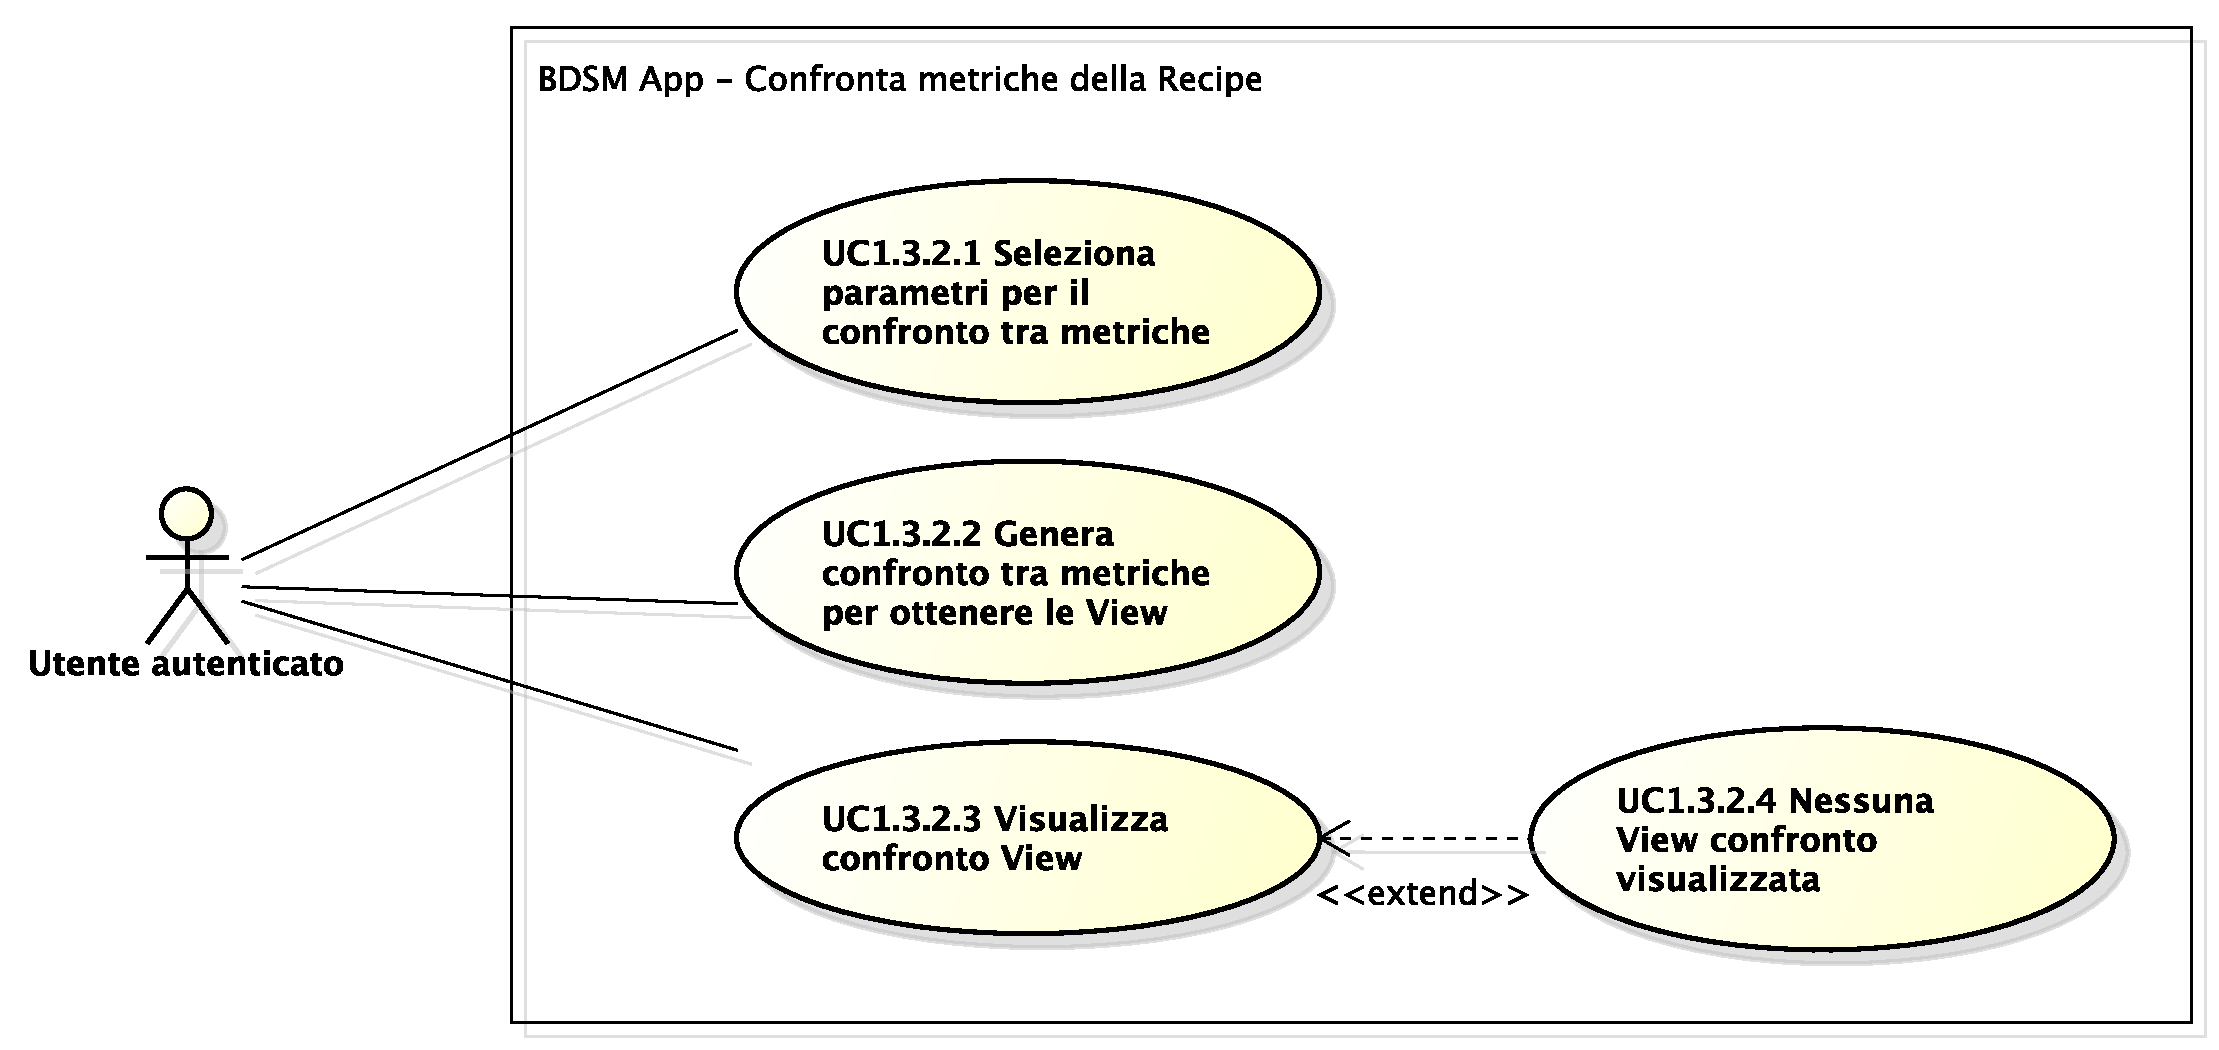
\includegraphics[scale=0.45]{./images/UC1_3_2.pdf}}
	\caption{UC1.3.1 - Confronta metriche della Recipe}
\end{figure}

\begin{itemize}
	\item \textbf{Attori:}
	\begin{itemize}
		\item utente autenticato: utente autenticato che ha accesso al servizio;
	\end{itemize}
	\item \textbf{Descrizione:} all'utente è stata fornita la possibilità di effettuare delle comparazioni tra le diverse metriche presenti in una Recipe. Questa comparazione potrà essere effettuata solo tra metriche equivalenti della stessa categoria (Facebook, Twitter, Instagram). Questo genererà delle View contenenti alcuni grafici e i relativi dati associati;
	\item \textbf{Precondizione:} l'utente è entrato nella sezione del confronto della Recipe selezionata;
	\item \textbf{Flusso principale degli eventi:}
		\begin{enumerate}
			\item Seleziona parametri per il confronto tra metriche (UC1.3.2.1);
			\item Genera confronto tra metriche per ottenere le View (UC1.3.2.2);
			\item Visualizza confronto View (UC1.3.2.3).
		\end{enumerate}
	\item \textbf{Postcondizione:} l'utente ha visualizzato le View relative alle metriche che ha deciso di confrontare;
	\item \textbf{Estensioni:} Nessuna View confronto visualizzata (UC1.3.2.4).

\end{itemize}
% FINE USE CASE %

\subsubsection{UC1.3.2.1: Seleziona parametri per il confronto tra metriche}
\begin{itemize}
	\item \textbf{Attori:}
	\begin{itemize}
		\item utente autenticato: utente autenticato che ha accesso al servizio;
	\end{itemize}
	\item \textbf{Descrizione:} per generare le View di confronto l'utente deve selezionare i parametri tra quelli disponibili dal sistema secondo un determinato ordine.
	\item \textbf{Precondizione:} l'utente è entrato nella sezione del confronto della Recipe selezionata;
	\item \textbf{Flusso principale degli eventi:}
	\begin{enumerate}
		\item Selezione categoria (UC1.3.2.1.1);
		\item Selezione tipo di metrica (UC1.3.2.1.2);
		\item Selezione metriche (UC1.3.2.1.3);
	\end{enumerate}
	\item \textbf{Postcondizione:} l'utente ha selezionato tutti i parametri richiesti per generare un confronto.
\end{itemize}
% FINE USE CASE %

\subsubsection{UC1.3.2.1.1: Selezione categoria}
\begin{itemize}
	\item \textbf{Attori:}
	\begin{itemize}
		\item utente autenticato: utente autenticato che ha accesso al servizio;
	\end{itemize}
	\item \textbf{Descrizione:} l'utente come primo passo deve selezionare la categoria tra le quali vuole cercare le metriche da confrontare. La categoria potrà essere scelta tra Facebook, Twitter, Instagram;
	\item \textbf{Precondizione:} l'utente è appena entrato nel pannello di confronto delle View e non ha ancora selezionato niente;
	\item \textbf{Scenario principale:} l'utente seleziona la categoria di metriche da confrontare;
	\item \textbf{Postcondizione:} l'utente ha selezionato la categoria tra quelle proposte.
\end{itemize}
% FINE USE CASE %

\subsubsection{UC1.3.2.1.2: Selezione tipo di metrica}
\begin{itemize}
	\item \textbf{Attori:}
	\begin{itemize}
		\item utente autenticato: utente autenticato che ha accesso al servizio;
	\end{itemize}
	\item \textbf{Descrizione:} l'utente, a seconda della categoria, avrà a disposizione delle tipologie di metriche tra le quali scegliere, in quanto per fare una View di confronto, ci vogliono dati equo comparabili;
	\item \textbf{Precondizione:} l'utente ha selezionato la categoria tra quelle proposte;
	\item \textbf{Scenario principale:} l'utente seleziona la tipologia di metrica che desidera confrontare;
	\item \textbf{Postcondizione:} l'utente ha selezionato la tipologia di metrica tra quelle proposte.
\end{itemize}
% FINE USE CASE %

\subsubsection{UC1.3.2.1.3: Selezione metriche}
\begin{itemize}
	\item \textbf{Attori:}
	\begin{itemize}
		\item utente autenticato: utente autenticato che ha accesso al servizio;
	\end{itemize}
	\item \textbf{Descrizione:} l'utente per generare le View relative al confronto deve almeno selezionare due metriche tra quelle proposte. Ne può selezionare anche un numero maggiore di due;
	\item \textbf{Precondizione:} l'utente ha selezionato la tipologia di metrica tra quelle proposte;
	\item \textbf{Scenario principale:} l'utente selezione le metriche che desidera confrontare;
	\item \textbf{Postcondizione:} l'utente ha selezionato almeno due metriche tra quelle proposte.
\end{itemize}
% FINE USE CASE %


\subsubsection{UC1.3.2.2: Genera confronto tra metriche per ottenere le View}
\begin{itemize}
	\item \textbf{Attori:}
	\begin{itemize}
		\item utente autenticato: utente autenticato che ha accesso al servizio;
	\end{itemize}
	\item \textbf{Descrizione:} per generare le View di confronto l'utente deve selezionare i parametri e premere sull'apposito pulsante;
	\item \textbf{Precondizione:} l'utente ha selezionato tutti i parametri richiesti per generare un confronto;
	\item \textbf{Scenario principale:} l'utente preme l'apposito pulsante per generare le View di confronto;
	\item \textbf{Postcondizione:} l'utente ha premuto sull'apposito pulsante per generare il confronto e creare le relative View.
\end{itemize}
% FINE USE CASE %

\subsubsection{UC1.3.2.3: Visualizza confronto View}
\begin{itemize}
	\item \textbf{Attori:}
	\begin{itemize}
		\item utente autenticato: utente autenticato che ha accesso al servizio;
	\end{itemize}
	\item \textbf{Descrizione:} l'utente andrà a visualizzare le View relative al confronto selezionato. Le View potranno contenere dei grafici quali Line Chart e Bar Chart, altrimenti potranno contenere dei dati in forma tabellare;
	\item \textbf{Precondizione:} l'utente ha premuto sull'apposito pulsante per generare il confronto e creare le relative View;
	\item \textbf{Scenario principale:} l'utente visualizza le View di confronto appena generate;
	\item \textbf{Postcondizione:} l'utente ha visualizzato le View che sono state generate dalla selezione.
\end{itemize}
% FINE USE CASE %

\subsubsection{UC1.3.2.4: Nessuna View confronto visualizzata}
\begin{itemize}
	\item \textbf{Attori:}
	\begin{itemize}
		\item utente autenticato: utente autenticato che ha accesso al servizio;
	\end{itemize}
	\item \textbf{Descrizione:} l'utente desidera visualizzare le View di confronto generate, ma i dati per generarle potrebbero essere ancora assenti qualora le metriche ricavate dalle Recipe fossero state inserite da poco nel sistema da parte degli amministratori;
	\item \textbf{Precondizione:} l'utente ha premuto sull'apposito pulsante per generare il confronto e creare le relative View;
	\item \textbf{Scenario principale:} l'utente visualizza un messaggio che lo informa che i dati per generare le View di confronto non sono ancora stati raccolti dal sistema;
	\item \textbf{Postcondizione:} l'utente ha preso atto dell'assenza di View di confronto per le metriche selezionate.
\end{itemize}
% FINE USE CASE %

\pagebreak


\subsection{UC1.4: Gestione delle Recipe}
\begin{figure}[!ht]
	\centering
	\centerline{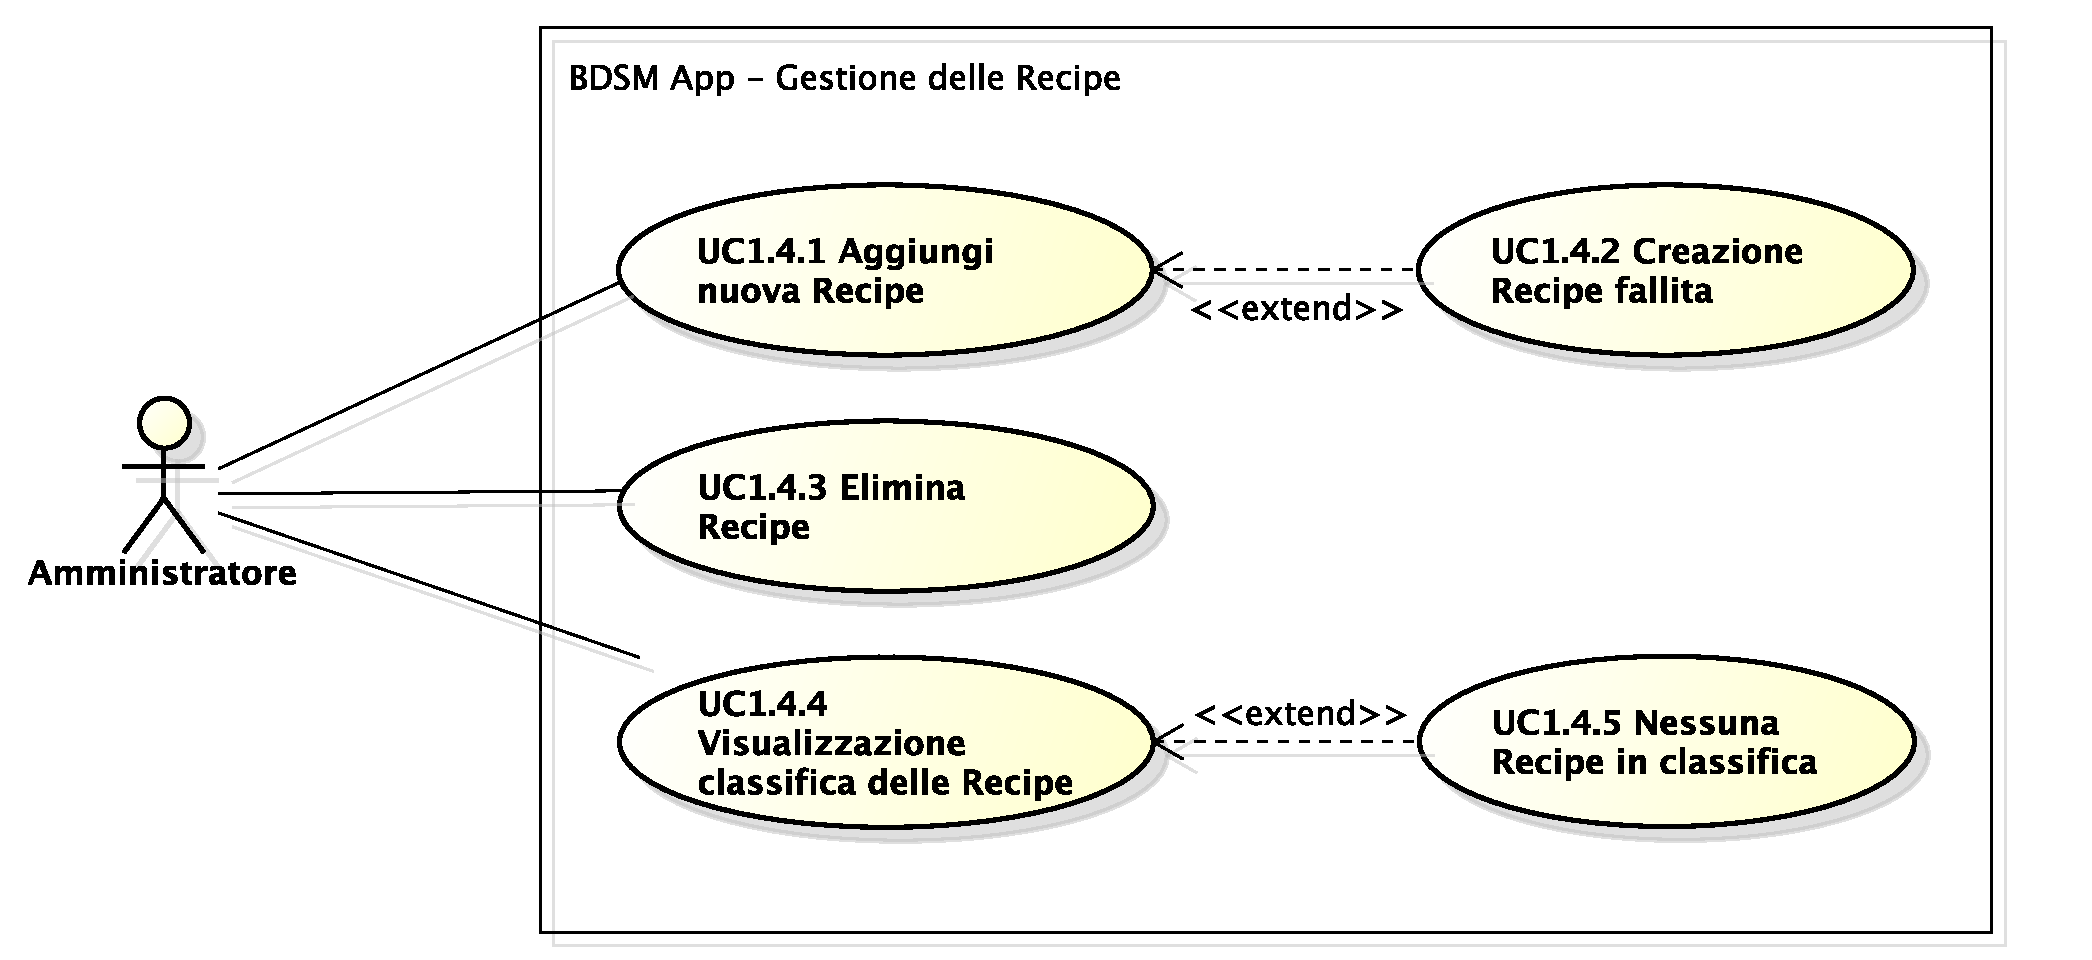
\includegraphics[scale=0.45]{./images/UC1_4.pdf}}
	\caption{UC1.4 - Gestione delle Recipe}
\end{figure}

\begin{itemize}
	\item \textbf{Attori:}
	\begin{itemize}
		\item utente amministratore: utente autenticato che ha accesso al servizio e dispone dei permessi per visualizzare tutte le aree;
	\end{itemize}
	\item \textbf{Descrizione:} gli amministratori possono vedere le Recipe e i dati ad esse associate. Possono inoltre crearle o eliminarle;
	\item \textbf{Precondizione:} l'amministratore autenticato è posizionato nella home screen dell'applicazione;
	\item \textbf{Flusso principale degli eventi:}
	\begin{enumerate}
		\item Visualizza Recipe (UC1.4.1);
		\item Aggiungi nuova Recipe (UC1.4.2);
		\item Elimina Recipe (UC1.4.4);
	\end{enumerate}
	\item \textbf{Postcondizione:} le informazioni richieste dall'amministratore sono state fornite, le Recipe eliminate, cancellate dal sistema e quelle aggiunte, salvate; Se durante la creazione sono stati inseriti valori che non rispettano i vincoli di sistema è stata visualizzata una schermata di errore;
	\item \textbf{Estensioni:} Creazione Recipe fallita (UC1.4.3).
\end{itemize}
% FINE USE CASE %

\subsubsection{UC1.4.2: Aggiungi nuova Recipe}
\begin{itemize}
	\item \textbf{Attori:}
	\begin{itemize}
		\item utente amministratore: utente autenticato che ha accesso al servizio e dispone dei permessi per visualizzare tutte le aree;
	\end{itemize}
	\item \textbf{Descrizione:} l'amministratore può aggiungere una nuova Recipe al sistema. Può scegliere il nome che la identificherà e ha a disposizione dei parametri per ogni social network che serviranno per fornire le indicazioni su che dati recuperare;
	\item \textbf{Precondizione:} l'amministratore è nella home page ed ha visualizzato l'elenco delle Recipe salvate nel sistema;
	\item \textbf{Flusso principale degli eventi:}
	\begin{enumerate}
		\item Apertura pannello inserimento nuova Recipe (UC1.4.2.1);
		\item Inserimento parametri (UC1.4.2.2);
		\item Conferma parametri inseriti (UC1.4.2.3).
	\end{enumerate}
	\item \textbf{Postcondizione:} l'amministratore ha salvato una nuova Recipe nel sistema;
\end{itemize}
% FINE USE CASE %

\subsubsection{UC1.4.2.1: Apertura pannello inserimento nuova Recipe}
\begin{itemize}
	\item \textbf{Attori:}
	\begin{itemize}
		\item utente amministratore: utente autenticato che ha accesso al servizio e dispone dei permessi per visualizzare tutte le aree;
	\end{itemize}
	\item \textbf{Descrizione:} l'amministratore può selezionare il pulsante di inserimento di una nuova Recipe dall'elenco delle Recipe;
	\item \textbf{Precondizione:} l'amministratore ha visualizzato l'elenco delle Recipe;
	\item \textbf{Scenario principale:} l'amministratore selezione il pulsante di inserimento nuove Recipe;
	\item \textbf{Postcondizione:} l'amministratore ha visualizzato il pannello di inserimento nuova Recipe.
\end{itemize}
% FINE USE CASE %

\subsubsection{UC1.4.2.2: Inserimento parametri}
\begin{itemize}
	\item \textbf{Attori:}
	\begin{itemize}
		\item utente amministratore: utente autenticato che ha accesso al servizio e dispone dei permessi per visualizzare tutte le aree;
	\end{itemize}
	\item \textbf{Descrizione:} l'amministratore può inserire il titolo, una breve descrizione ed i parametri relativi alle metriche delle diverse categorie per poter portare a compimento la creazione di una nuova Recipe;
	\item \textbf{Precondizione:} l'amministratore ha selezionato il pulsante per l'inserimento di una nuova Recipe;
	\item \textbf{Flusso principale degli eventi:}
	\begin{enumerate}
		\item Inserimento titolo Recipe (UC1.4.2.3.1);
		\item Inserimento descrizione Recipe (UC1.4.2.3.2);
		\item Inserimento metrica (UC1.4.2.3.3);
	\end{enumerate}
	\item \textbf{Postcondizione:} l'amministratore ha inserito tutti i parametri richiesti dal sistema.
\end{itemize}
% FINE USE CASE %

\subsubsection{UC1.4.2.2.1: Inserimento titolo Recipe}
\begin{itemize}
	\item \textbf{Attori:}
	\begin{itemize}
		\item utente amministratore: utente autenticato che ha accesso al servizio e dispone dei permessi per visualizzare tutte le aree;
	\end{itemize}
	\item \textbf{Descrizione:} l'amministratore deve obbligatoriamente inserire il titolo che identifica la Recipe che sta per andare a inserire nel sistema;
	\item \textbf{Precondizione:} l'amministratore si trova nel pannello di inserimento nuova Recipe;
	\item \textbf{Scenario principale:} l'amministratore inserisce il titolo della Recipe;
	\item \textbf{Postcondizione:} l'amministratore ha inserito il titolo della Recipe.
\end{itemize}
% FINE USE CASE %

\subsubsection{UC1.4.2.2.2: Inserimento descrizione Recipe}
\begin{itemize}
	\item \textbf{Attori:}
	\begin{itemize}
		\item utente amministratore: utente autenticato che ha accesso al servizio e dispone dei permessi per visualizzare tutte le aree;
	\end{itemize}
	\item \textbf{Descrizione:} l'amministratore ha la possibilità di aggiungere una piccola descrizione alla Recipe che sta per inserire in modo da potere dare qualche nota che lo aiuti in futuro a capirne al meglio la natura. L'amministratore può decidere di lasciare il campo vuoto;
	\item \textbf{Precondizione:} l'amministratore si trova nel pannello di inserimento nuova Recipe;
	\item \textbf{Scenario principale:} l'amministratore inserisce una descrizione della Recipe o lascia il campo vuoto;
	\item \textbf{Postcondizione:} l'amministratore ha inserito una descrizione della Recipe o ha lasciato il campo vuoto.
\end{itemize}
% FINE USE CASE %

\subsubsection{UC1.4.2.2.3: Inserimento metrica}
\begin{itemize}
	\item \textbf{Attori:}
	\begin{itemize}
		\item utente amministratore: utente autenticato che ha accesso al servizio e dispone dei permessi per visualizzare tutte le aree;
	\end{itemize}
	\item \textbf{Descrizione:} per generare una Recipe, l'amministratore deve inserire i parametri che consentono al sistema di andare a recuperare i dati necessari. Questa operazione deve essere effettuato almeno una volta;
	\item \textbf{Precondizione:} l'amministratore non ha ancora inserito una metrica o ne ha già inserita una completa ed ora desidera inserirne un'altra;
	\item \textbf{Scenario principale:} l'amministratore inserisce tutti i valori richiesti;
	\item \textbf{Postcondizione:} l'amministratore ha inserito tutti i valori richiesti o ha lasciato i campi vuoti.
\end{itemize}
% FINE USE CASE %



\subsubsection{UC1.4.2.4: Conferma parametri inseriti}
\begin{itemize}
	\item \textbf{Attori:}
	\begin{itemize}
		\item utente amministratore: utente autenticato che ha accesso al servizio e dispone dei permessi per visualizzare tutte le aree;
	\end{itemize}
	\item \textbf{Descrizione:} l'amministratore deve confermare i parametri inseriti prima che questi siano attivi nel sistema;
	\item \textbf{Precondizione:} l'amministratore ha inserito almeno i parametri obbligatori;
	\item \textbf{Scenario principale:} l'amministratore preme il pulsante di conferma creazione Recipe;
	\item \textbf{Postcondizione:} l'amministratore ha confermato i parametri inseriti.
\end{itemize}
% FINE USE CASE %

\subsubsection{UC1.4.3: Creazione Recipe fallita}
\begin{itemize}
	\item \textbf{Attori:}
	\begin{itemize}
		\item utente amministratore: utente autenticato che ha accesso al servizio e dispone dei permessi per visualizzare tutte le aree;
	\end{itemize}
	\item \textbf{Descrizione:} l'amministratore durante l'inserimento di una nuova Recipe ha inserito dei parametri non conformi alle specifiche presenti in UC1.4.2.3 o non ha inserito almeno uno metrica (nel complessivo, non almeno una per categoria);
	\item \textbf{Precondizione:} l'amministratore ha selezionato il pulsante di conferma per la creazione di una nuova Recipe;
	\item \textbf{Scenario principale:} l'amministratore ha visualizzato un messaggio di errore contenente l'elenco dei parametri inseriti non corretti o un messaggio che dice che manca da inserire almeno una metrica;
	\item \textbf{Postcondizione:} l'amministratore ha preso atto che i dati inseriti non sono corretti o sufficienti per la creazione delle Recipe.
\end{itemize}
% FINE USE CASE %

\subsubsection{UC1.4.4: Eliminazione Recipe}
\begin{itemize}
	\item \textbf{Attori:}
	\begin{itemize}
		\item utente amministratore: utente autenticato che ha accesso al servizio e dispone dei permessi per visualizzare tutte le aree;
	\end{itemize}
	\item \textbf{Descrizione}: l'amministratore può eliminare una Recipe e tutti i dati ad essa associati;
	\item \textbf{Precondizione:} l'amministratore deve aver visualizzato la schermata di gestione delle Recipe;
	\item \textbf{Flusso principale degli eventi:}
	\begin{enumerate}
		\item Eliminazione Recipe (UC1.4.4.1);
		\item Conferma eliminazione Recipe (UC1.4.4.2).
	\end{enumerate}
	\item \textbf{Postcondizione:} le informazioni richieste dall'utente sono state fornite e la Recipe desiderata, con tutti i dati ad essa associati sono stati eliminati dal sistema;
\end{itemize}
% FINE USE CASE %

\subsubsection{UC1.4.4.1: Eliminazione Recipe}
\begin{itemize}
	\item \textbf{Attori:}
	\begin{itemize}
		\item utente amministratore: utente autenticato che ha accesso al servizio e dispone dei permessi per visualizzare tutte le aree;
	\end{itemize}
	\item \textbf{Descrizione:} l'amministratore può selezionare il pulsante di eliminazione di una Recipe nell'elenco delle Recipe;
	\item \textbf{Precondizione:} l'amministratore ha visualizzato l'elenco delle Recipe;
	\item \textbf{Scenario principale:} l'amministratore ha selezionato il pulsante di eliminazione di una Recipe;
	\item \textbf{Postcondizione:} l'amministratore ha selezionato il pulsante di eliminazione di una Recipe.
\end{itemize}
% FINE USE CASE %

\subsubsection{UC1.4.4.2: Conferma eliminazione Recipe}
\begin{itemize}
	\item \textbf{Attori:}
	\begin{itemize}
		\item utente amministratore: utente autenticato che ha accesso al servizio e dispone dei permessi per visualizzare tutte le aree;
	\end{itemize}
	\item \textbf{Descrizione:} l'amministratore deve confermare la volontà di eliminare la Recipe selezionando il pulsante di conferma eliminazione;
	\item \textbf{Precondizione:} l'amministratore ha selezionato il pulsante elimina su una Recipe;
	\item \textbf{Scenario principale:} l'amministratore conferma l'eliminazione delle Recipe;
	\item \textbf{Postcondizione:} l'amministratore ha confermato l'eliminazione della Recipe e questa è stata cancellata dal sistema con a tutti i dati associati.
\end{itemize}
% FINE USE CASE %

\pagebreak


\subsection{UC1.5: Modifica password di accesso}
\begin{figure}[!htbp]
	\centering
	\centerline{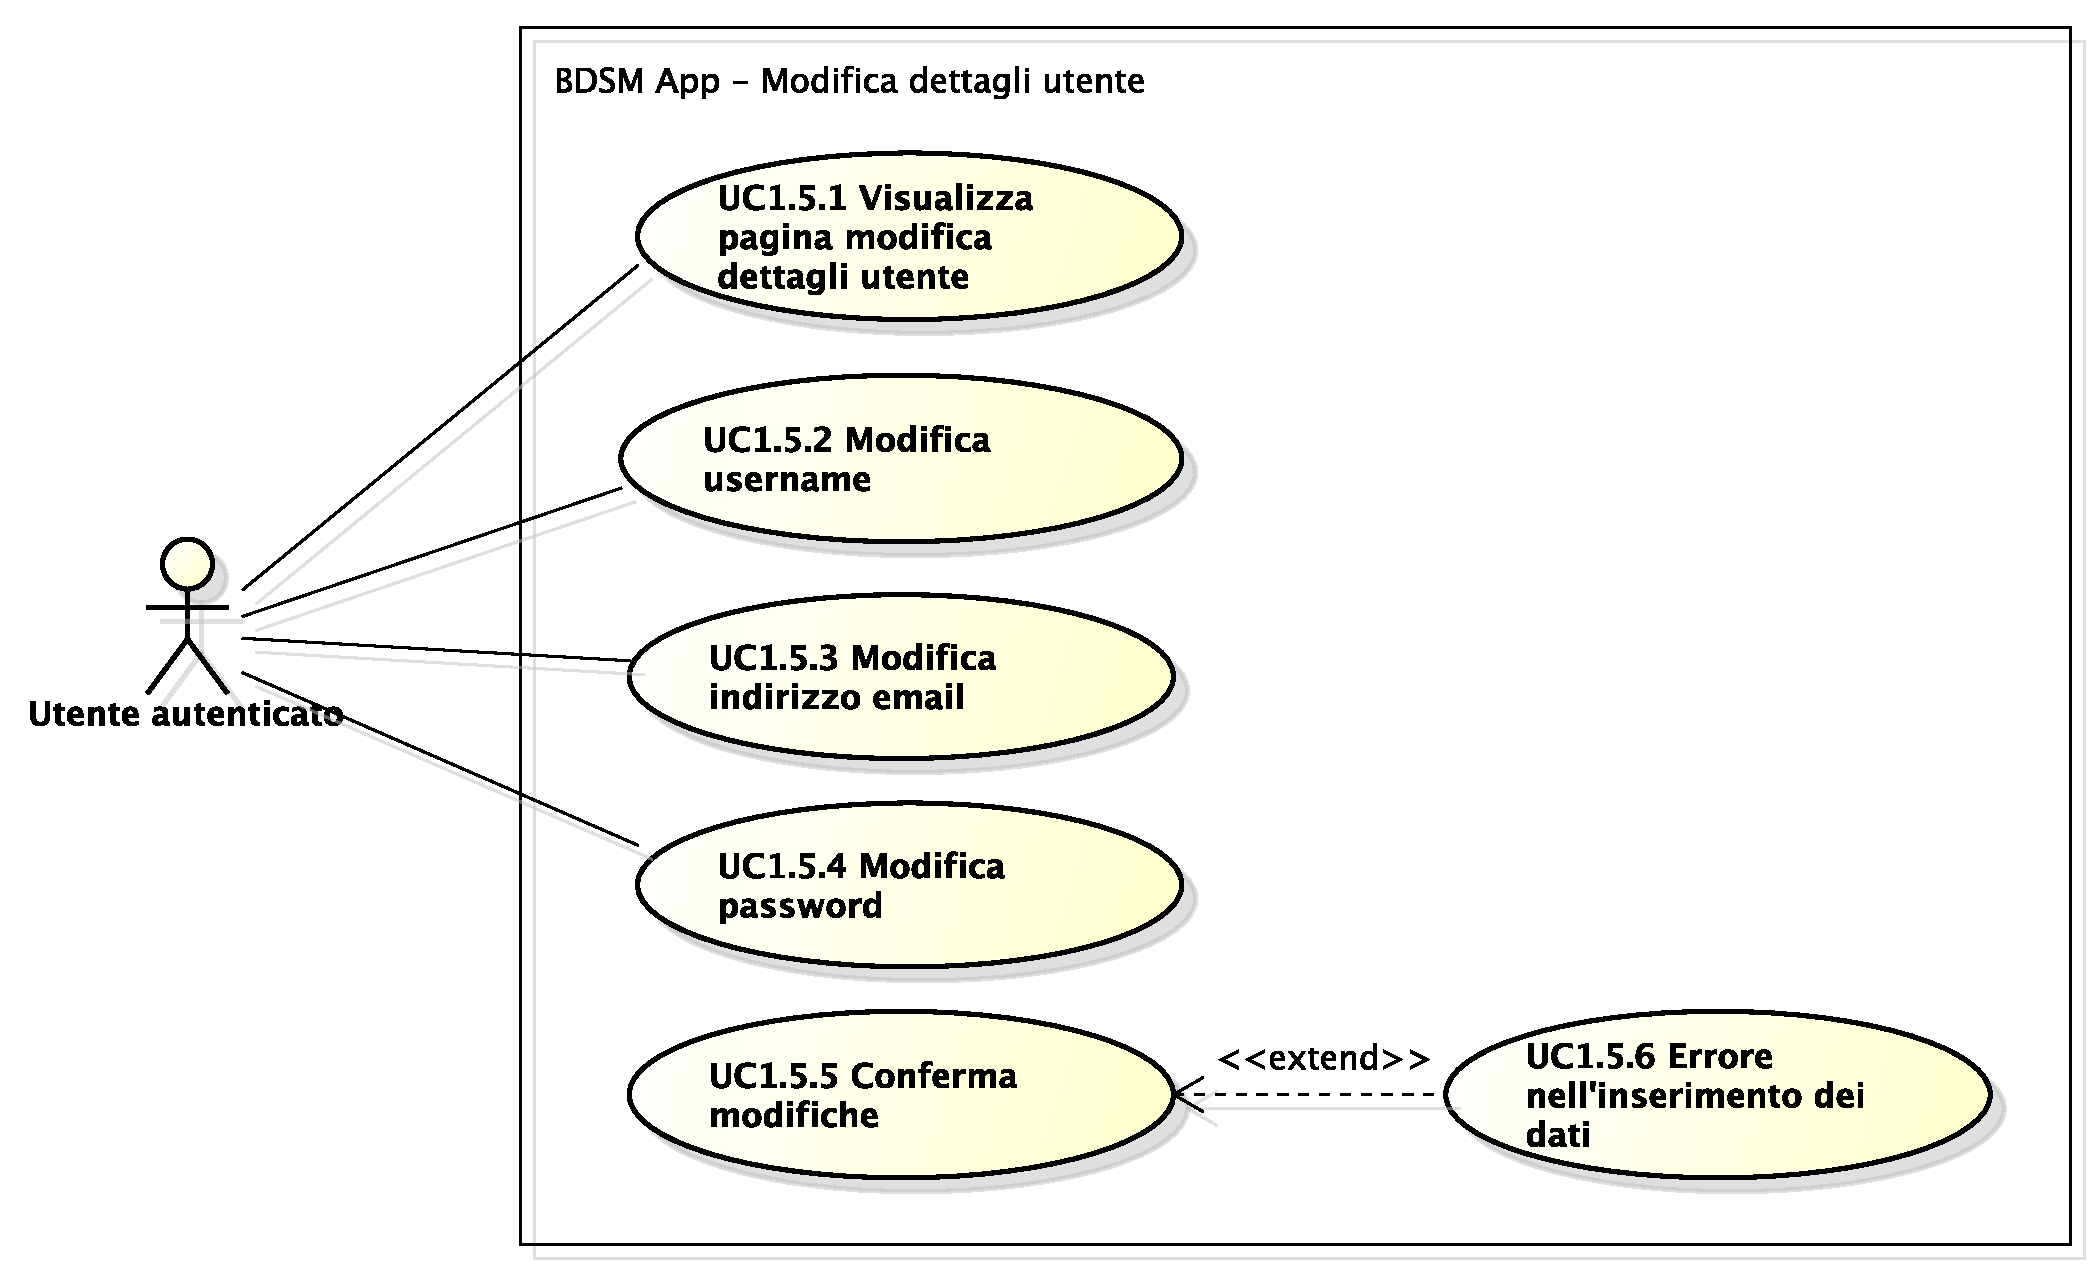
\includegraphics[scale=0.45]{./images/UC1_5.pdf}}
	\caption{UC1.5 - Modifica password di accesso}
\end{figure}

\begin{itemize}
	\item \textbf{Attori:}
	\begin{itemize}
		\item utente autenticato: utente autenticato che ha accesso al servizio;
	\end{itemize}
	\item \textbf{Descrizione:} l'utente può cambiare la propria password selezionando il pulsante di cambio password nel pannello utente;
	\item \textbf{Precondizione:} l'utente dispone di una password di accesso valida, risulta autenticato al servizio e si trova nel pannello utente;
	\item \textbf{Flusso principale degli eventi:}
	\begin{enumerate}
		\item Inserimento nuova password (UC1.5.1);
		\item Conferma inserimento nuova password (UC1.5.2);
		\item Inserimento vecchia password (UC1.5.3);
		\item Conferma cambio password (UC1.5.4);
	\end{enumerate}
	\item \textbf{Postcondizione:} la nuova password per l'utente è attiva, la vecchia password non è più valida;
	\item \textbf{Estensioni:} Vecchia password inserita non valida (UC1.5.5).
\end{itemize}
% FINE USE CASE %

\subsubsection{UC1.5.1: Inserimento nuova password}
\begin{itemize}
	\item \textbf{Attori:}
	\begin{itemize}
		\item utente autenticato: utente autenticato che ha accesso al servizio;
	\end{itemize}
	\item \textbf{Descrizione:} l'utente può inserire la nuova password nel pannello apposito;
	\item \textbf{Precondizione:} l'utente ha selezionato il pulsante di cambio password nella sua home screen;
	\item \textbf{Scenario principale:} l'utente inserisce la nuova password nell'apposito campo;
	\item \textbf{Postcondizione:} l'utente ha inserito la nuova password.
\end{itemize}

\subsubsection{UC1.5.2: Conferma inserimento password }
\begin{itemize}
	\item \textbf{Attori:}
	\begin{itemize}
		\item utente autenticato: utente autenticato che ha accesso al servizio;
	\end{itemize}
	\item \textbf{Descrizione:} l'utente deve inserire nuovamente la nuova password per verificare di non aver fatto errori di battitura;
	\item \textbf{Precondizione:} l'utente ha inserito la nuova password;
	\item \textbf{Scenario principale:} l'utente inserisce la password di conferma nell'apposito campo;
	\item \textbf{Postcondizione:} l'utente ha verificato la correttezza della nuova password.
\end{itemize}
% FINE USE CASE %

\subsubsection{UC1.5.3: Inserimento vecchia password}
\begin{itemize}
	\item \textbf{Attori:}
	\begin{itemize}
		\item utente autenticato: utente autenticato che ha accesso al servizio;
	\end{itemize}
	\item \textbf{Descrizione:} l'utente deve inserire la vecchia password per completare il cambio password;
	\item \textbf{Precondizione:} l'utente ha inserito la nuova password due volte negli appositi campi;
	\item \textbf{Scenario principale:} l'utente inserisce la vecchia password nell'apposito campo;
	\item \textbf{Postcondizione:} l'utente ha inserito la vecchia password e può confermare la nuova.
\end{itemize}
% FINE USE CASE %

\subsubsection{UC1.5.4: Conferma cambio password}
\begin{itemize}
	\item \textbf{Attori:}
	\begin{itemize}
		\item utente autenticato: utente autenticato che ha accesso al servizio;
	\end{itemize}
	\item \textbf{Descrizione:} l'utente deve confermare di voler sostituire la vecchia password di accesso con quella nuova selezionando il pulsante di conferma;
	\item \textbf{Precondizione:} l'utente ha inserito due volte la nuova password ed una la vecchia negli appositi campi;
	\item \textbf{Scenario principale:} l'utente preme il pulsante di conferma cambio password;
	\item \textbf{Postcondizione:} l'utente ha confermato l'operazione e la nuova password è ora attiva.
\end{itemize}
% FINE USE CASE %

\subsubsection{UC1.5.5: Password non corretta}
\begin{itemize}
	\item \textbf{Attori:}
	\begin{itemize}
		\item utente autenticato: utente autenticato che ha accesso al servizio;
	\end{itemize}
	\item \textbf{Descrizione:} l'utente può aver inserito una password che non soddisfa i vincoli di sistema specificati nel pannello di cambio password;
	\item \textbf{Precondizione:} l'utente ha selezionato il pulsante di conferma del cambio password;
	\item \textbf{Scenario principale:} l'utente visualizza un messaggio di errore con i dettagli dei vincoli non soddisfatti;
	\item \textbf{Postcondizione:} l'utente ha preso atto che i dati inseriti non sono validi e per quali motivazioni.
\end{itemize}
% FINE USE CASE %

\pagebreak


\subsection{UC1.6: Logout utente}
\begin{figure}[htbp]
	\centering
	\centerline{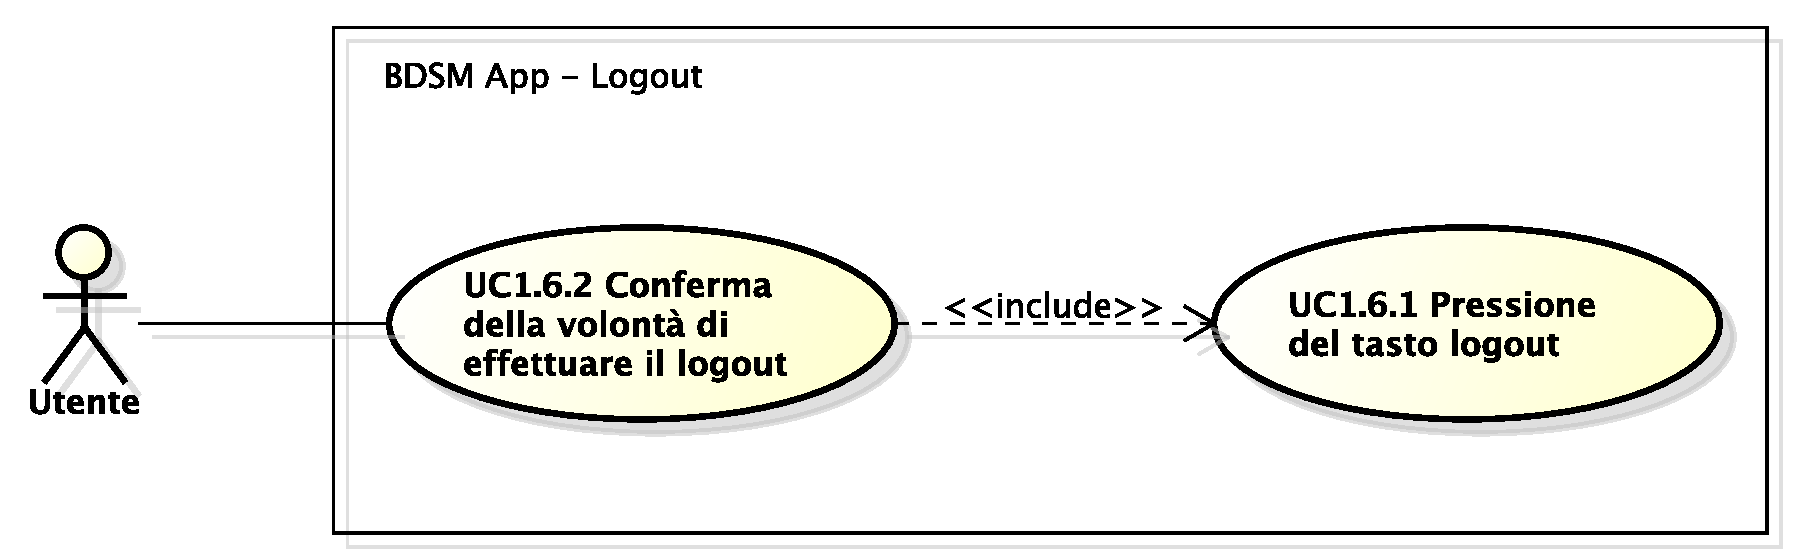
\includegraphics[scale=0.45]{./images/UC1_6.pdf}}
	\caption{UC1.6 - Logout utente}
\end{figure}

\begin{itemize}
	\item \textbf{Attori:}
	\begin{itemize}
		\item utente autenticato: utente autenticato che ha accesso al servizio;
	\end{itemize}
	\item \textbf{Descrizione:} l'utente può terminare la sessione di lavoro. Questa operazione può essere eseguita premendo il pulsante di logout nella home screen;
	\item \textbf{Precondizione:} l'utente risulta autenticato al servizio;
	\item \textbf{Flusso principale degli eventi:}
	\begin{enumerate}
		\item Pressione tasto logout (UC1.6.1);
		\item Conferma del logout (UC1.6.2).
	\end{enumerate}
	\item \textbf{Postcondizione:} la sessione di lavoro è terminata. Viene mostrata la schermata di login;
\end{itemize}
% FINE USE CASE %

\subsubsection{UC1.6.1: Pressione tasto logout}
\begin{itemize}
	\item \textbf{Attori:}
	\begin{itemize}
		\item utente autenticato: utente autenticato che ha accesso al servizio;
	\end{itemize}
	\item \textbf{Descrizione:} l'utente può effettuare il logout selezionando l'apposito pulsante nella sua home screen;
	\item \textbf{Precondizione:} l'utente ha effettuato l'accesso al servizio e si trova nella home screen;
	\item \textbf{Scenario principale:} l'utente preme l'apposito pulsante di logout;
	\item \textbf{Postcondizione:} l'utente visualizza il pannello di conferma logout.
\end{itemize}
% FINE USE CASE %

\subsubsection{UC1.6.2: Conferma del logout}
\begin{itemize}
	\item \textbf{Attori:}
	\begin{itemize}
		\item utente autenticato: utente autenticato che ha accesso al servizio;
	\end{itemize}
	\item \textbf{Descrizione:} prima di terminare la sessione di lavoro l'utente deve confermare la volontà di farlo selezionando il pulsante di conferma sul pannello di logout;
	\item \textbf{Precondizione:} l'utente ha selezionato il pulsante di logout nella home screen;
	\item \textbf{Scenario principale:} l'utente preme l'apposito pulsante per la conferma del logout;
	\item \textbf{Postcondizione:} l'utente ha confermato il logout e la sessione è terminata.
\end{itemize}
% FINE USE CASE %

\pagebreak


\subsection{UC1.7: Amministrazione degli utenti}
\begin{figure}[!htbp]
	\centering
	\centerline{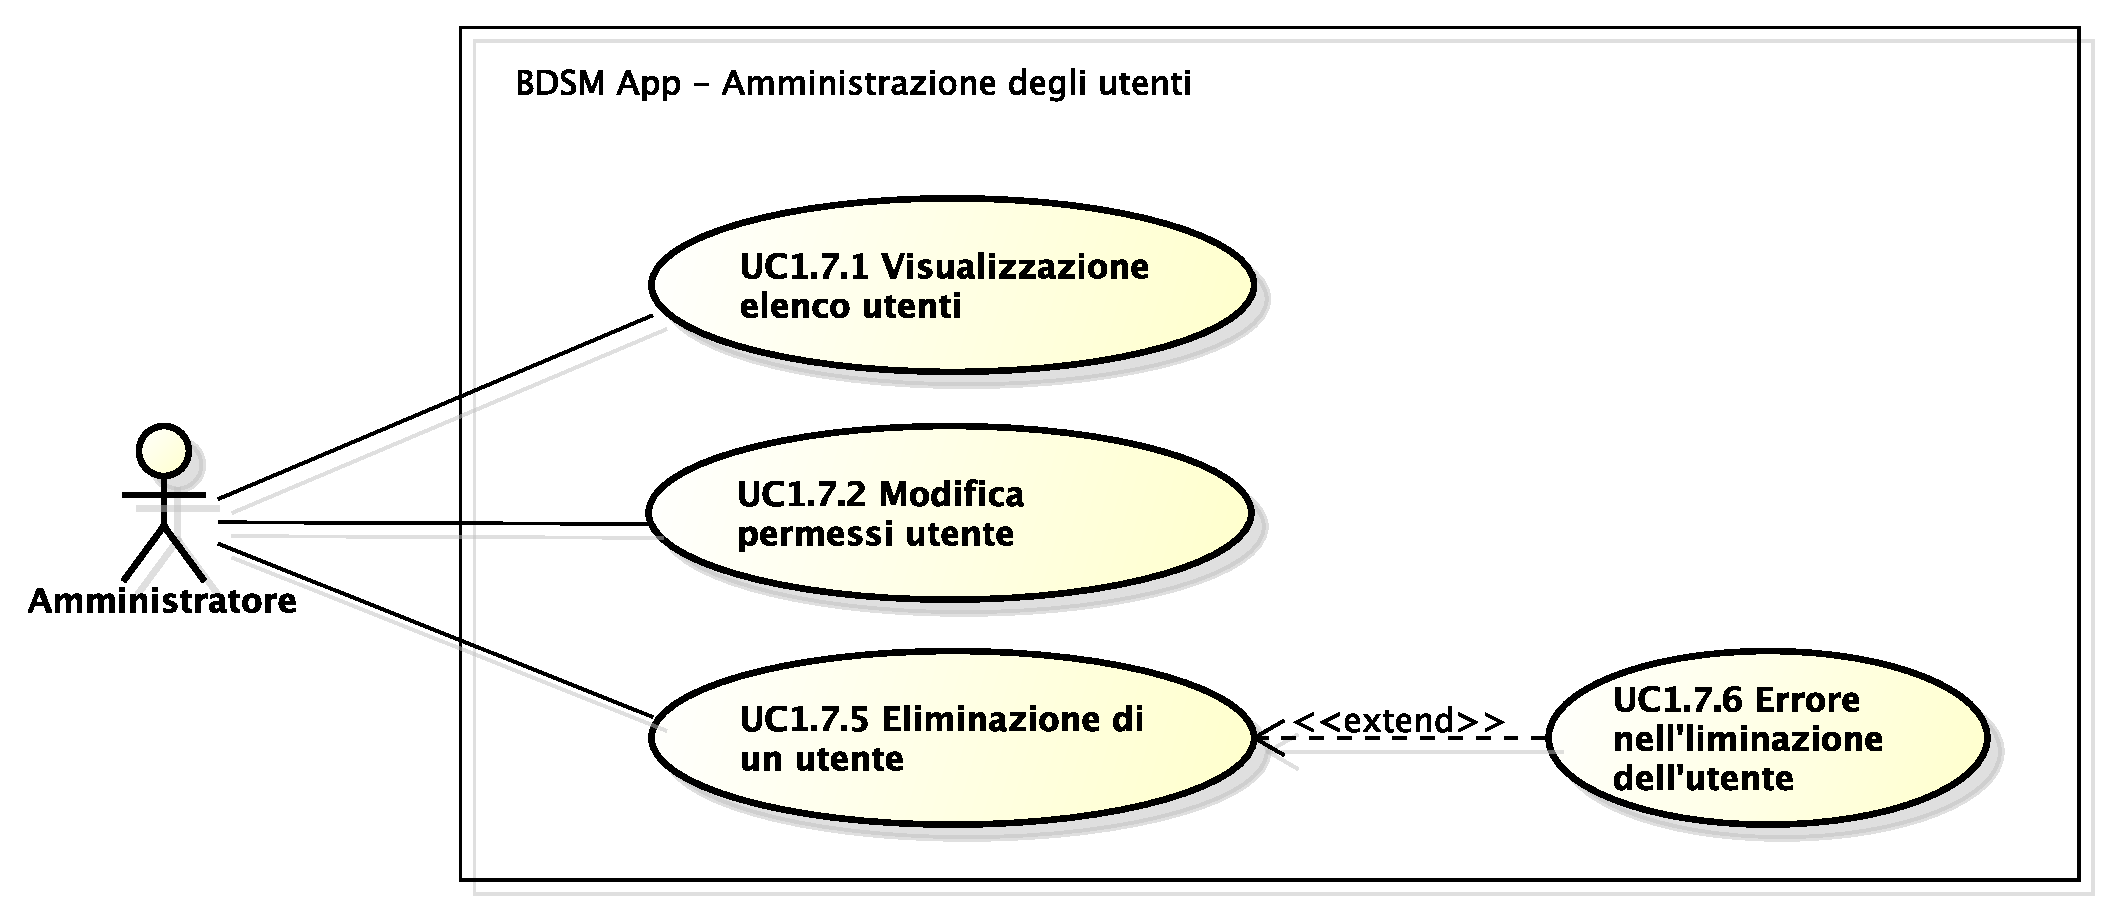
\includegraphics[scale=0.45]{./images/UC1_7.pdf}}
	\caption{UC1.7 - Amministrazioni degli utenti}
\end{figure}

\begin{itemize}
	\item \textbf{Attori:}
	\begin{itemize}
		\item utente amministratore: utente autenticato che ha accesso al servizio e dispone dei permessi per visualizzare tutte le aree;
	\end{itemize}
	\item \textbf{Descrizione:} l'amministratore può gestire i permessi di accesso di un altro utente o eliminarlo definitivamente del sistema;
	\item \textbf{Precondizione:} l'amministratore ha effettuato l'accesso al sistema;
	\item \textbf{Flusso principale degli eventi:}
	\begin{enumerate}
		\item Visualizzazione elenco utenti (UC1.7.1);
		\item Modifica permessi utente (UC1.7.2);
		\item Eliminazione utente (UC1.7.3);
		\item Conferma modifiche (UC1.7.4).
	\end{enumerate}
	\item \textbf{Postcondizione:} il sistema ha eseguito le operazioni richieste;
	\item \textbf{Estensioni:} Errore nella gestione degli utenti (UC1.7.5).
\end{itemize}
% FINE USE CASE %

\subsubsection{UC1.7.1: Visualizzazione elenco utenti}
\begin{itemize}
	\item \textbf{Attori:}
	\begin{itemize}
		\item utente amministratore: utente autenticato che ha accesso al servizio e dispone dei permessi per visualizzare tutte le aree;
	\end{itemize}
	\item \textbf{Descrizione:} l'amministratore può visualizzare l'elenco di tutti gli utenti salvati nel sistema selezionando l'apposito pulsante nella home screen;
	\item \textbf{Precondizione:} l'amministratore ha effettuato l'accesso al sistema e si trova nella home screen;
	\item \textbf{Scenario principale:} l'amministratore seleziona l'apposito pulsate per visualizzare la lista degli utenti registrati al sistema;
	\item \textbf{Postcondizione:} l'amministratore ha visualizzato l'elenco degli utenti.
\end{itemize}
% FINE USE CASE %

\subsubsection{UC1.7.2: Modifica permessi utente}
\begin{itemize}
	\item \textbf{Attori:}
	\begin{itemize}
		\item utente amministratore: utente autenticato che ha accesso al servizio e dispone dei permessi per visualizzare tutte le aree;
	\end{itemize}
	\item \textbf{Descrizione:} l'amministratore può abilitare o disabilitare i permessi di amministratore ad un utente diverso da se stesso;
	\item \textbf{Precondizione:} l'amministratore ha eseguito l'accesso ed ha visualizzato l'elenco degli utenti;
	\item \textbf{Scenario principale:} l'amministratore preme l'apposito pulsante per modificare i permessi di un utente;
	\item \textbf{Postcondizione:} l'amministratore ha modificato i permessi ad un utente;
\end{itemize}
% FINE USE CASE %

\subsubsection{UC1.7.3: Eliminazione utente}
\begin{itemize}
	\item \textbf{Attori:}
	\begin{itemize}
		\item utente amministratore: utente autenticato che ha accesso al servizio e dispone dei permessi per visualizzare tutte le aree;
	\end{itemize}
	\item \textbf{Descrizione:} l'amministratore può eliminare un utente da sistema;
	\item \textbf{Precondizione:} l'amministratore ha eseguito l'accesso ed ha visualizzato l'elenco degli utenti;
	\item \textbf{Scenario principale:} l'amministratore preme l'apposito pulsate per la rimozione di un utente;
	\item \textbf{Postcondizione:} l'amministratore ha cancellato un utente dal sistema;
\end{itemize}
% FINE USE CASE %

\subsubsection{UC1.7.4: Conferma modifiche}
\begin{itemize}
	\item \textbf{Attori:}
	\begin{itemize}
		\item utente amministratore: utente autenticato che ha accesso al servizio e dispone dei permessi per visualizzare tutte le aree;
	\end{itemize}
	\item \textbf{Descrizione:} l'amministratore deve confermare le modifiche apportate agli utenti;
	\item \textbf{Precondizione:} l'amministratore ha effettuato delle modiche nella pagina di elenco utenti;
	\item \textbf{Scenario principale:} l'amministratore preme l'apposito pulsate per la conferma delle modifiche;
	\item \textbf{Postcondizione:} l'amministratore ha confermato le modifiche e sono ora attive nel sistema.
\end{itemize}
% FINE USE CASE %

\subsubsection{UC1.7.5: Errore nella gestione degli utenti}
\begin{itemize}
	\item \textbf{Attori:}
	\begin{itemize}
		\item utente amministratore: utente autenticato che ha accesso al servizio e dispone dei permessi per visualizzare tutte le aree;
	\end{itemize}
	\item \textbf{Descrizione:} l’amministratore può visualizzare un messaggio di errore se l’utente che vuole eliminare è attualmente autenticato al sistema e sta eseguendo delle operazioni o in caso stia cercando di modificare i permessi di sè stesso;
	\item \textbf{Precondizione:} l'amministratore ha confermato le modifiche apportate;
	\item \textbf{Scenario principale:} l'amministratore visualizza un messaggio contentente gli errori rilevati dal sistema;
	\item \textbf{Postcondizione:} l'amministratore ha preso atto degli errori effettuati.
\end{itemize}
% FINE USE CASE %

\pagebreak


\subsection{UC1.8: Registrazione nuovo utente}
\begin{figure}[!htbp]
	\centering
	\centerline{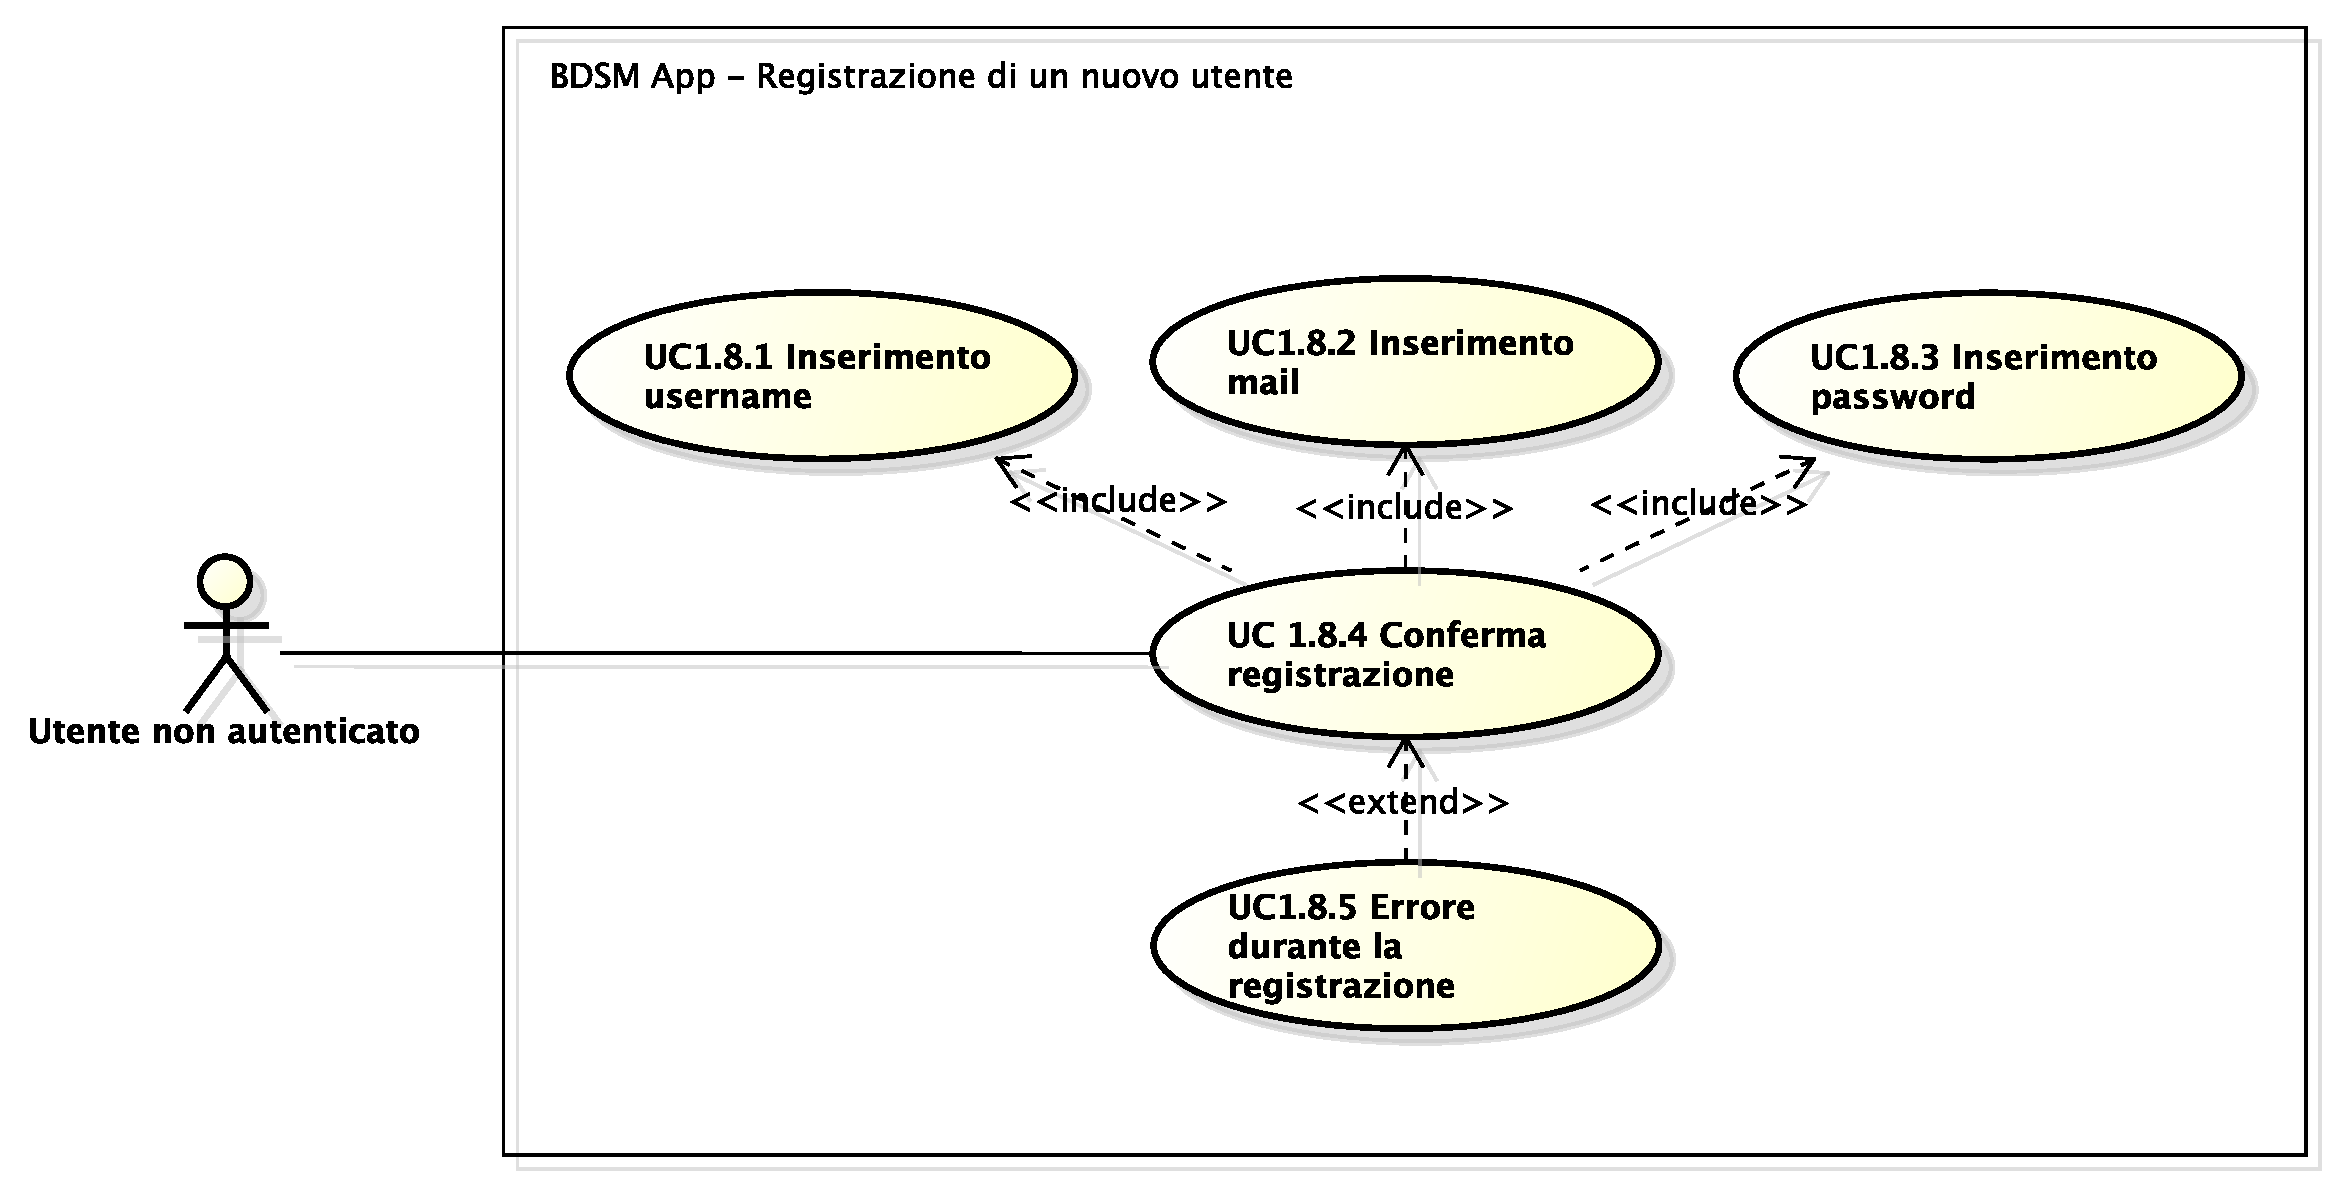
\includegraphics[scale=0.45]{./images/UC1_8.pdf}}
	\caption{UC1.8 - Registrazione nuovo utente}
\end{figure}

\begin{itemize}
	\item \textbf{Attori:}
	\begin{itemize}
		\item utente non autenticato: utente non ancora noto al sistema che accede al servizio;
	\end{itemize}
	\item \textbf{Descrizione:} un utente deve poter creare un account per poter eseguire il login
	all'interno del sistema e usufruire delle funzionalità offerte;
	\item \textbf{Precondizione:} l'utente accede al sito web tramite un browser supportato
	dal sistema;
	\item \textbf{Flusso principale degli eventi:}
	\begin{enumerate}
		\item Inserimento username (UC1.8.1);
		\item Inserimento email (UC1.8.2);
		\item Inserimento password (UC1.8.3);
		\item Conferma registrazione (UC1.8.4);
	\end{enumerate}
	\item \textbf{Postcondizione:} il sistema ha memorizzato i dati relativi al nuovo account e
	ripresenta all'utente la schermata iniziale;
	\item \textbf{Estensioni:} Creazione utente fallita (UC1.8.5).
\end{itemize}
% FINE USE CASE %

\subsubsection{UC1.8.1: Inserimento username}
\begin{itemize}
	\item \textbf{Attori:}
	\begin{itemize}
		\item utente non autenticato: utente non ancora noto al sistema che accede al servizio;
	\end{itemize}
	\item \textbf{Descrizione:} l'utente deve inserire il proprio nome utente in modo da essere riconoscibile univocamente all'interno del sistema e per poter gestire i relativi dati associati;
	\item \textbf{Precondizione:} il sistema fornisce una schermata in cui è possibile inserire l'username per il nuovo account;
	\item \textbf{Scenario principale:} l'utente inserisce lo username nell'apposito campo;
	\item \textbf{Postcondizione:} l'utente ha inserito il proprio username.
\end{itemize}
% FINE USE CASE %

\subsubsection{UC1.8.2: Inserimento mail}
\begin{itemize}
	\item \textbf{Attori:}
	\begin{itemize}
		\item utente non autenticato: utente non ancora noto al sistema che accede al servizio;
	\end{itemize}
	\item \textbf{Descrizione:} l'utente deve inserire la mail che vuole associare alle username appena inserito;
	\item \textbf{Precondizione:} il sistema fornisce una schermata in cui è possibile inserire la mail per il nuovo account;
	\item \textbf{Scenario principale:} l'utente inserisce il proprio indirizzo mail nell'apposito campo;
	\item \textbf{Postcondizione:} l'utente ha inserito il proprio indirizzo mail.
\end{itemize}
% FINE USE CASE %

\subsubsection{UC1.8.3: Inserimento password}
\begin{itemize}
	\item \textbf{Attori:}
	\begin{itemize}
		\item utente non autenticato: utente non ancora noto al sistema che accede al servizio;
	\end{itemize}
	\item \textbf{Descrizione:} l'utente deve inserire la password che vuole associare ai dati precedentemente inseriti;
	\item \textbf{Precondizione:} il sistema fornisce una schermata in cui è possibile inserire la password per il nuovo account;
	\item \textbf{Scenario principale:} l'utente ha inserito la password nell'apposito campo;
	\item \textbf{Postcondizione:} l'utente ha inserito la password.
\end{itemize}
% FINE USE CASE %

\subsubsection{UC1.8.3: Inserimento password di conferma}
\begin{itemize}
	\item \textbf{Attori:}
	\begin{itemize}
		\item utente non autenticato: utente non ancora noto al sistema che accede al servizio;
	\end{itemize}
	\item \textbf{Descrizione:} l'utente deve inserire la password di conferma uguale a quella inserita precedentemente;
	\item \textbf{Precondizione:} il sistema fornisce una schermata in cui è possibile inserire la password una seconda volta;
	\item \textbf{Scenario principale:} l'utente ha inserito la password di conferma nell'apposito campo;
	\item \textbf{Postcondizione:} l'utente ha inserito la password di conferma.
\end{itemize}
% FINE USE CASE %

\subsubsection{UC1.8.4: Conferma registrazione}
\begin{itemize}
	\item \textbf{Attori:}
	\begin{itemize}
		\item utente non autenticato: utente non ancora noto al sistema che accede al servizio;
	\end{itemize}
	\item \textbf{Descrizione:} l'utente deve poter confermare i dati inseriti durante la registrazione;
	\item \textbf{Precondizione:} il sistema fornisce una schermata in cui è possibile confermare i dati inseriti in precedenza per la creazione di un nuovo account;
	\item \textbf{Scenario principale:} l'utente seleziona l'apposito pulsante di conferma dei dati inseriti;
	\item \textbf{Postcondizione:} l'utente ha confermato di voler creare un nuovo account all'interno del sistema.
\end{itemize}
% FINE USE CASE %

\subsubsection{UC1.8.5: Errore durante la registrazione}
\begin{itemize}
	\item \textbf{Attori:}
	\begin{itemize}
		\item utente non autenticato: utente non ancora noto al sistema che accede al servizio;
	\end{itemize}
	\item \textbf{Descrizione:} se vengono inseriti dei dati non conformi ai vincoli di sistema indicati durante la registrazione viene visualizzata una schermata di errore;
	\item \textbf{Precondizione:} i dati inseriti non rispettano uno o più vincoli di sistema;
	\item \textbf{Scenario principale:} l'utente visualizza un messaggio di errore che indica gli errori riscontrati nei dati inseriti;
	\item \textbf{Postcondizione:} l'utente ha preso atto degli errori effettuati.
\end{itemize}
% FINE USE CASE %

\pagebreak

\subsection{UC1.9: Richiesta aggiunta Recipe}
\begin{figure}[!htbp]
	\centering
	\centerline{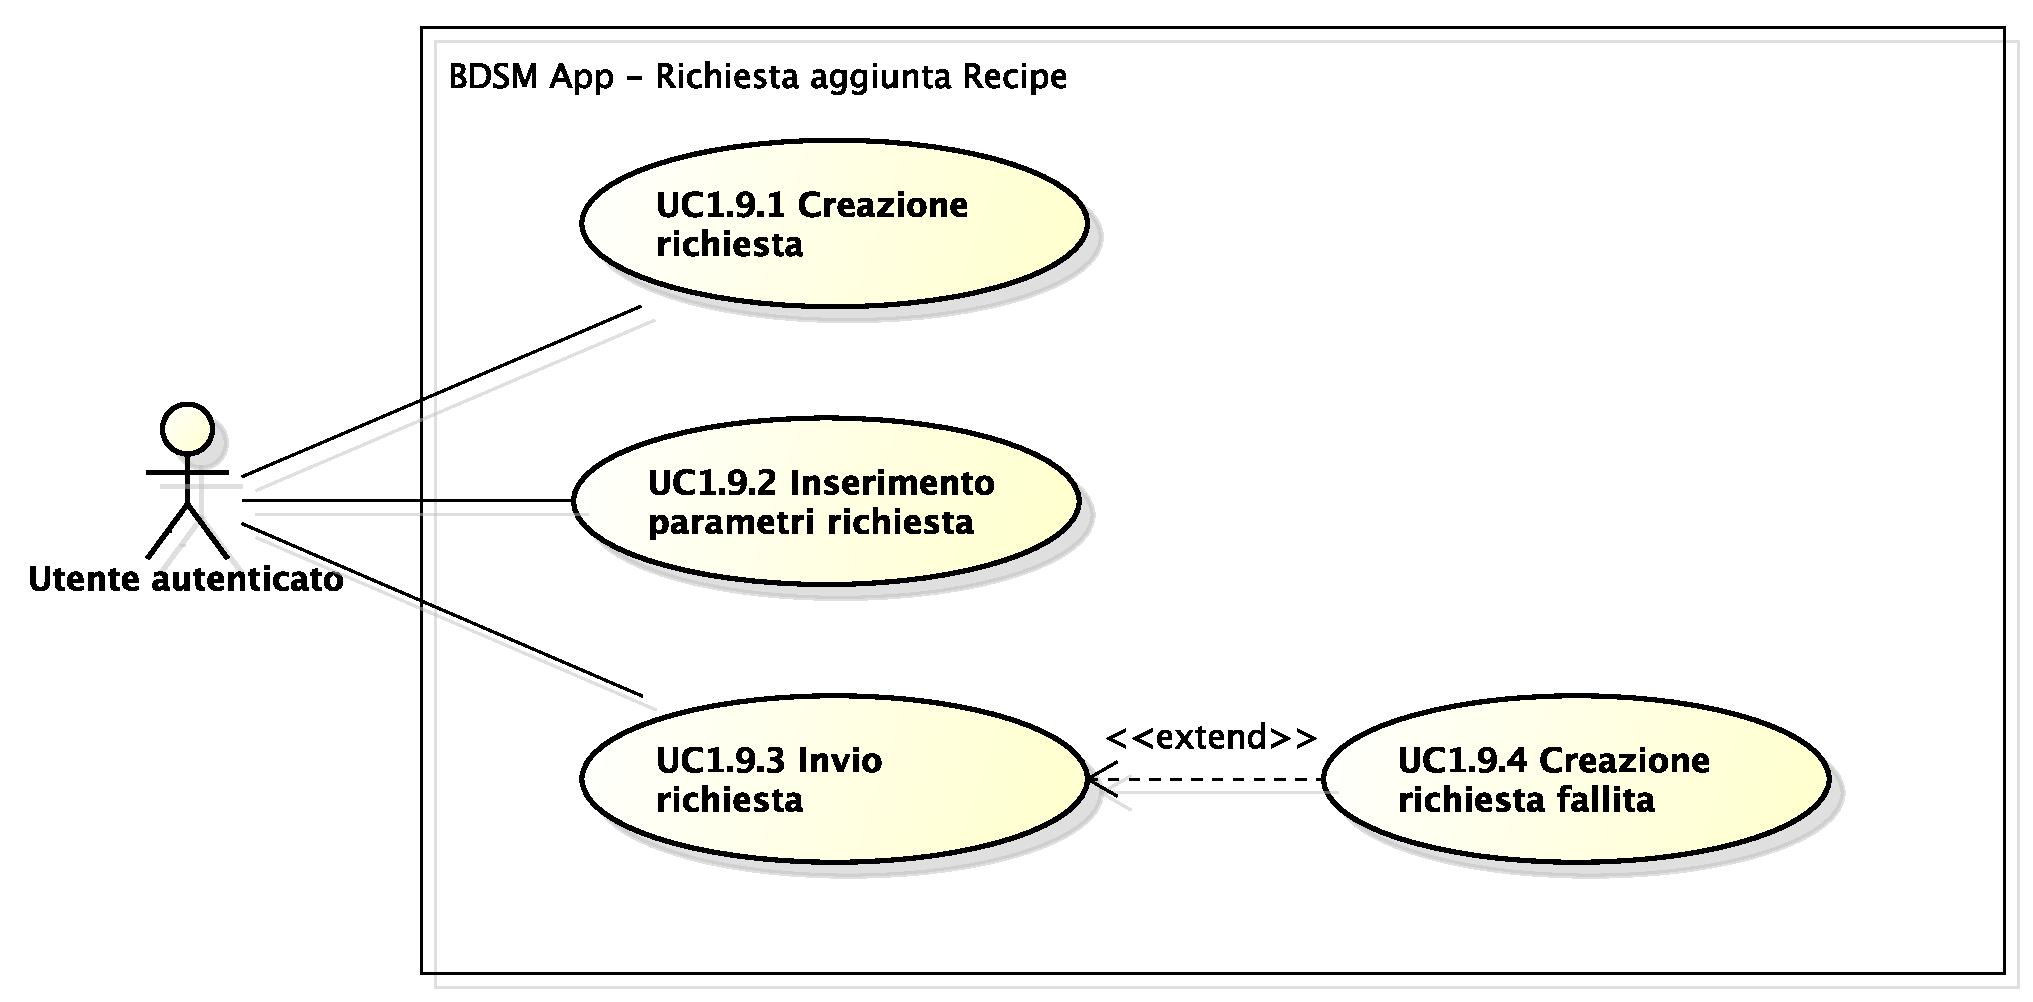
\includegraphics[scale=0.50]{./images/UC1_9.pdf}}
	\caption{UC1.9 - Richiesta aggiunta Recipe}
\end{figure}

\begin{itemize}
	\item \textbf{Attori:}
	\begin{itemize}
		\item utente autenticato: utente autenticato che ha accesso al servizio;
	\end{itemize}
	\item \textbf{Descrizione:} l'utente può richiedere agli amministratori di aggiungere una nuova Recipe e relative View al sistema utilizzando l'apposito form nella WebGUI;
	\item \textbf{Precondizione:} l'utente ha effettuato l'accesso al sistema;
	\item \textbf{Flusso principale degli eventi:}
	\begin{enumerate}
		\item Creazione richiesta (UC1.9.1);
		\item Inserimento parametri richiesta (UC1.9.2);
		\item Invio richiesta (UC1.9.3);
	\end{enumerate}
	\item \textbf{Postcondizione:} la richiesta è stata inoltrata agli amministratori;
	\item \textbf{Estensioni:} Creazione richiesta fallita (UC1.9.4).
\end{itemize}
% FINE USE CASE %

\subsubsection{UC1.9.1: Creazione richiesta}
\begin{itemize}
	\item \textbf{Attori:}
	\begin{itemize}
		\item utente autenticato: utente che ha effettuato l'accesso nell'applicazione;
	\end{itemize}
	\item \textbf{Descrizione:} l'utente può accedere al pannello per la creazione di una richiesta di aggiunta Recipe da inviare agli amministratori, che valuteranno se accettarla o meno;
	\item \textbf{Precondizione:} l'utente ha effettuato l'accesso al sistema e si trova nella home screen;
	\item \textbf{Scenario principale:} l'utente seleziona l'apposito pulsante di richiesta View;
	\item \textbf{Postcondizione:} l'utente ha visualizzato il pannello per effettuare una richiesta di inserimento di una nuova Recipe.

\end{itemize}
% FINE USE CASE %

\subsubsection{UC1.9.2: Inserimento parametri richiesta}
\begin{itemize}
	\item \textbf{Attori:}
	\begin{itemize}
		\item utente autenticato: utente che ha effettuato l'accesso nell'applicazione;
	\end{itemize}
	\item \textbf{Descrizione:} l'utente, una volta entrato nell'apposito pannello, per completare una richiesta per una nuova Recipe, deve compilare tutti i campi richiesti dal form;
	\item \textbf{Precondizione:} l'utente ha visualizzato il pannello per l'inserimento dei dati richiesti;
	\item \textbf{Scenario principale:} l'utente inserisce i dati necessari ad inviare la richiesta;
	\item \textbf{Postcondizione:} l'utente ha inserito tutti i parametri richiesti dal pannello.
\end{itemize}
% FINE USE CASE %

\subsubsection{UC1.9.3: Invio richiesta}
\begin{itemize}
	\item \textbf{Attori:}
	\begin{itemize}
		\item utente autenticato: utente che ha effettuato l'accesso nell'applicazione;
	\end{itemize}
	\item \textbf{Descrizione:} una volta che l'utente ha compilato tutti i campi richiesti dal pannello, può inviare la richiesta in maniera che venga valutata;
	\item \textbf{Precondizione:} l'utente ha inserito tutti i parametri richiesti;
	\item \textbf{Scenario principale:} l'utente preme sull'apposito pulsante per inviare la richiesta;
	\item \textbf{Postcondizione:} l'utente visualizza la conferma dell'avvenuto invio della richiesta.
\end{itemize}
% FINE USE CASE %

\subsubsection{UC1.9.4: Creazione richiesta fallita}
\begin{itemize}
	\item \textbf{Attori:}
	\begin{itemize}
		\item utente autenticato: utente che ha effettuato l'accesso nell'applicazione;
	\end{itemize}
	\item \textbf{Descrizione:} la creazione di una richiesta può fallire qualora i dati richiesti da inserire non fossero conformi alle attese;
	\item \textbf{Precondizione:} l'utente ha inserito tutti i parametri richiesti e ha premuto sull'apposito bottone per l'invio;
	\item \textbf{Scenario principale:} l'utente visualizza un errore che indica che indica quali parametri inseriti non sono corretti;
	\item \textbf{Postcondizione:} l'utente ha preso atto degli errori effettuati;
\end{itemize}
% FINE USE CASE %

\pagebreak


\subsection{UC1.10: Gestione richieste Recipe}
\begin{figure}[htbp]
	\centering
	\centerline{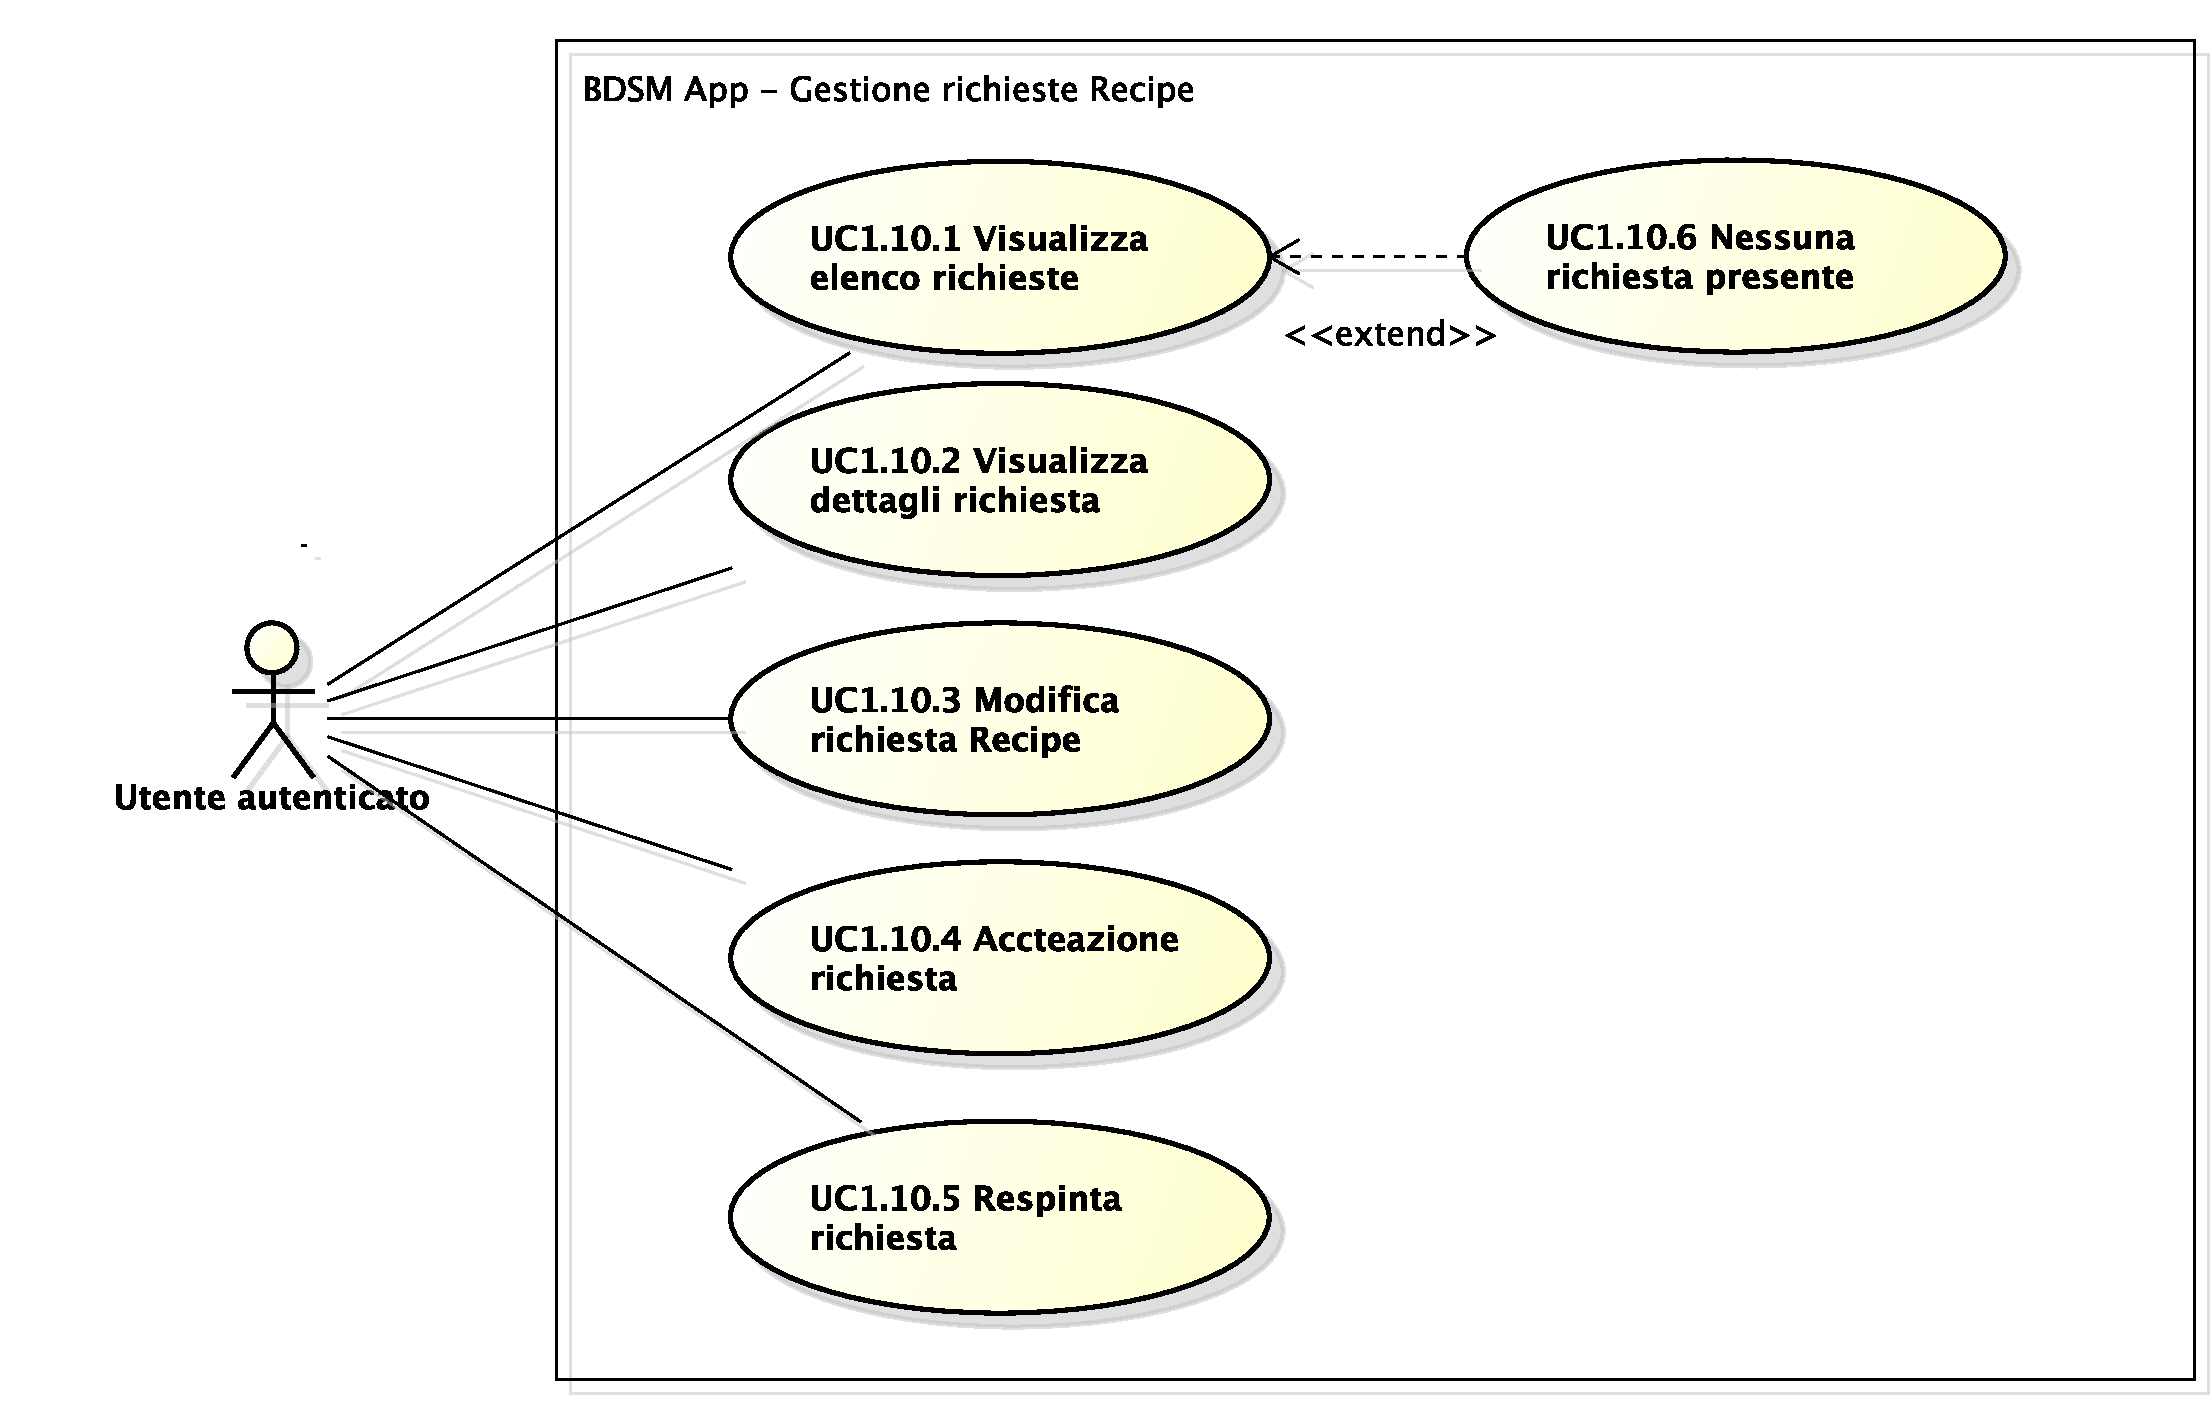
\includegraphics[scale=0.50]{./images/UC1_10.pdf}}
	\caption{UC1.10 - Gestione richieste Recipe}
\end{figure}

\begin{itemize}
	\item \textbf{Attori:}
	\begin{itemize}
		\item utente amministratore: utente autenticato che ha accesso al servizio e dispone dei permessi per visualizzare tutte le aree;
	\end{itemize}
	\item \textbf{Descrizione:} gli amministratori possono vedere tutte le richieste di aggiunta Recipe inviate correttamente dagli utenti. Possono inoltre marcare una richiesta come ```chiusa'' qualora sia stata accettata oppure rifiutata;
	\item \textbf{Precondizione:} l'amministratore dopo essersi autenticato ha selezionato il pulsante di gestione richieste utente dal menu principale dell'applicazione;
	\item \textbf{Flusso principale degli eventi:}
	\begin{enumerate}
		\item Visualizza elenco richieste (UC1.10.1);
		\item Visualizza dettagli richiesta (UC1.10.2);
		\item Modifica richiesta (UC1.10.3);
		\item Accettazione richiesta (UC1.10.4);
		\item Respinta richiesta (UC1.10.5);
	\end{enumerate}
	\item \textbf{Postcondizione:} le informazioni richieste dall'amministratore sono state fornite, le richiesta marcate come chiuse non sono più visibili nell'elenco;
	\item \textbf{Estensioni:} Nessuna richiesta presente (UC1.10.6).
\end{itemize}
% FINE USE CASE %

\subsubsection{UC1.10.1: Visualizza elenco richieste}
	\begin{itemize}
		\item \textbf{Attori:}
		\begin{itemize}
			\item utente amministratore: utente autenticato che ha accesso al servizio e dispone dei permessi per visualizzare tutte le aree;
		\end{itemize}
		\item \textbf{Descrizione:} l'amministratore può visualizzare un elenco delle richieste per delle nuove Recipe che sono state inviate dagli utenti normali e non ancore ``chiuse'';
		\item \textbf{Precondizione:} devono essere presenti delle richieste di nuove Recipe. L'amministratore desidera visualizzare le richieste ricevute;
		\item \textbf{Scenario principale:} l'amministratore selezione l'apposito pulsante per visualizzare le Recipe;
		\item \textbf{Postcondizione:} l'amministratore ha visualizzato l'elenco delle richieste di nuove Recipe.
	\end{itemize}
% FINE USE CASE %

\subsubsection{UC1.10.2: Visualizza dettagli richiesta}
	\begin{itemize}
		\item \textbf{Attori:}
		\begin{itemize}
			\item utente amministratore: utente autenticato che ha accesso al servizio e dispone dei permessi per visualizzare tutte le aree;
		\end{itemize}
		\item \textbf{Descrizione:} l'amministratore può visualizzare la richiesta che ha selezionato per controllarne i parametri;
		\item \textbf{Precondizione:} l'amministratore ha visualizzato l'elenco delle richieste;
		\item \textbf{Scenario principale:} l'amministratore ha selezionato l'apposito pulsante per la visualizzazione dei dettagli della richiesta;
		\item \textbf{Postcondizione:} l'amministratore ha visualizzato i dettagli della richiesta.
	\end{itemize}
% FINE USE CASE %

\subsubsection{UC1.10.3: Modifica richiesta Recipe}
	\begin{itemize}
		\item \textbf{Attori:}
		\begin{itemize}
			\item utente amministratore: utente autenticato che ha accesso al servizio e dispone dei permessi per visualizzare tutte le aree;
		\end{itemize}
		\item \textbf{Descrizione:} l'amministratore può modificare alcuni parametri della richiesta per renderla più efficace da comprendere;
		\item \textbf{Precondizione:} l'amministratore è entrato nella visualizzazione dei dettagli della richiesta;
		\item \textbf{Flusso principale degli eventi:}
		\begin{enumerate}
			\item Modifica titolo Recipe (UC1.10.3.1);
			\item Modifica descrizione Recipe (UC1.10.3.2);
		\end{enumerate}
		\item \textbf{Postcondizione:} l'amministratore ha modificato alcuni parametri delle richiesta;
	\end{itemize}
% FINE USE CASE %

\subsubsection{UC1.10.3.1: Modifica titolo Recipe}
	\begin{itemize}
		\item \textbf{Attori:}
		\begin{itemize}
			\item utente amministratore: utente autenticato che ha accesso al servizio e dispone dei permessi per visualizzare tutte le aree;
		\end{itemize}
		\item \textbf{Descrizione:} l'amministratore può decidere di modificare il titolo della Recipe richiesta per renderlo più comprensibile e utile;
		\item \textbf{Precondizione:} l'amministratore controlla il titolo inserito dall'utente per la Recipe e riscontra qualche mancanza o poca chiarezza di comprensione;
		\item \textbf{Scenario principale:} l'amministratore modifica il titolo della Recipe richiesta;
		\item [TO DO] (possibile scenario alternativo se l'amministratore non modifica nulla ?)
		\item \textbf{Postcondizione:} l'amministratore ha modificato il titolo.
	\end{itemize}
% FINE USE CASE %

\subsubsection{UC1.10.3.2: Modifica descrizione Recipe}
	\begin{itemize}
		\item \textbf{Attori:}
		\begin{itemize}
			\item utente amministratore: utente autenticato che ha accesso al servizio e dispone dei permessi per visualizzare tutte le aree;
		\end{itemize}
		\item \textbf{Descrizione:} l'amministratore può decidere di modificare la descrizione della Recipe richiesta per renderla più comprensibile e utile, o di inserirla qualora non fosse stata specificata dall'utente richiedente;
		\item \textbf{Precondizione:} l'amministratore controlla la descrizione inserita dall'utente per la Recipe e riscontra qualche mancanza, poca chiarezza di comprensione o assenza del campo;
		\item \textbf{Scenario principale:} l'amministratore modifica la descrizione della Recipe richiesta;
		\item [TO DO] (possibile scenario alternativo se l'amministratore non modifica nulla ?)
		\item \textbf{Postcondizione:} l'amministratore ha modificato la descrizione.
	\end{itemize}
% FINE USE CASE %

\subsubsection{UC1.10.4: Accettazione richiesta}
	\begin{itemize}
		\item \textbf{Attori:}
		\begin{itemize}
			\item utente amministratore: utente autenticato che ha accesso al servizio e dispone dei permessi per visualizzare tutte le aree;
		\end{itemize}
		\item \textbf{Descrizione:} l'amministratore una volta controllata la bontà della Recipe richiesta potrà accettarla in modo che venga inserita nel sistema;
		\item \textbf{Precondizione:} l'amministratore sta visualizzando in dettaglio la Recipe che decide di inserire nel sistema;
		\item \textbf{Scenario principale:} l'amministratore preme l'apposito pulsante per confermare l'accettazione della Recipe;
		\item \textbf{Postcondizione:} l'amministratore visualizza un messaggio di conferma inserimento e la Recipe è stata inserita nel sistema.
	\end{itemize}
% FINE USE CASE %

\subsubsection{UC1.10.5: Respinta richiesta}
	\begin{itemize}
		\item \textbf{Attori:}
		\begin{itemize}
			\item utente amministratore: utente autenticato che ha accesso al servizio e dispone dei permessi per visualizzare tutte le aree;
		\end{itemize}
		\item \textbf{Descrizione:} l'amministratore una volta controllata la richiesta per una nuova Recipe potrà decidere di rifiutarla qualora non ritenesse opportuno il suo inserimento nel sistema;
		\item \textbf{Precondizione:} l'amministratore seleziona l'apposito pulsante per respingere la richiesta di inserimento Recipe;
		\item \textbf{Scenario principale:} l'amministratore preme l'apposito pulsante per respingere la richiesta della Recipe;
		\item \textbf{Postcondizione:} l'amministratore visualizza un messaggio di conferma e ha può immettere una motivazione da inviare all'utente;
	\end{itemize}
% FINE USE CASE %

\subsubsection{UC1.10.6: Nessuna richiesta presente}
	\begin{itemize}
		\item \textbf{Attori:}
		\begin{itemize}
			\item utente amministratore: utente autenticato che ha accesso al servizio e dispone dei permessi per visualizzare tutte le aree;
		\end{itemize}
		\item \textbf{Descrizione:} non sono state effettuate richiesta di nuove Recipe da parte degli utenti;
		\item \textbf{Precondizione:} l'amministratore seleziona l'apposito pulsante per visualizzare le richieste di inserimento Recipe;
		\item \textbf{Scenario principale:} l'amministratore dopo avere premuto sul pulsante per visualizzare le richieste di Recipe, non ne trova neanche una presente;
		\item \textbf{Postcondizione:} l'amministratore visualizza un messaggio che non sono presenti richieste di Recipe;
	\end{itemize}
% FINE USE CASE %




\pagebreak


\subsection{UC1.11: Gestione dei preferiti}
\begin{figure}[htbp]
	\centering
	\centerline{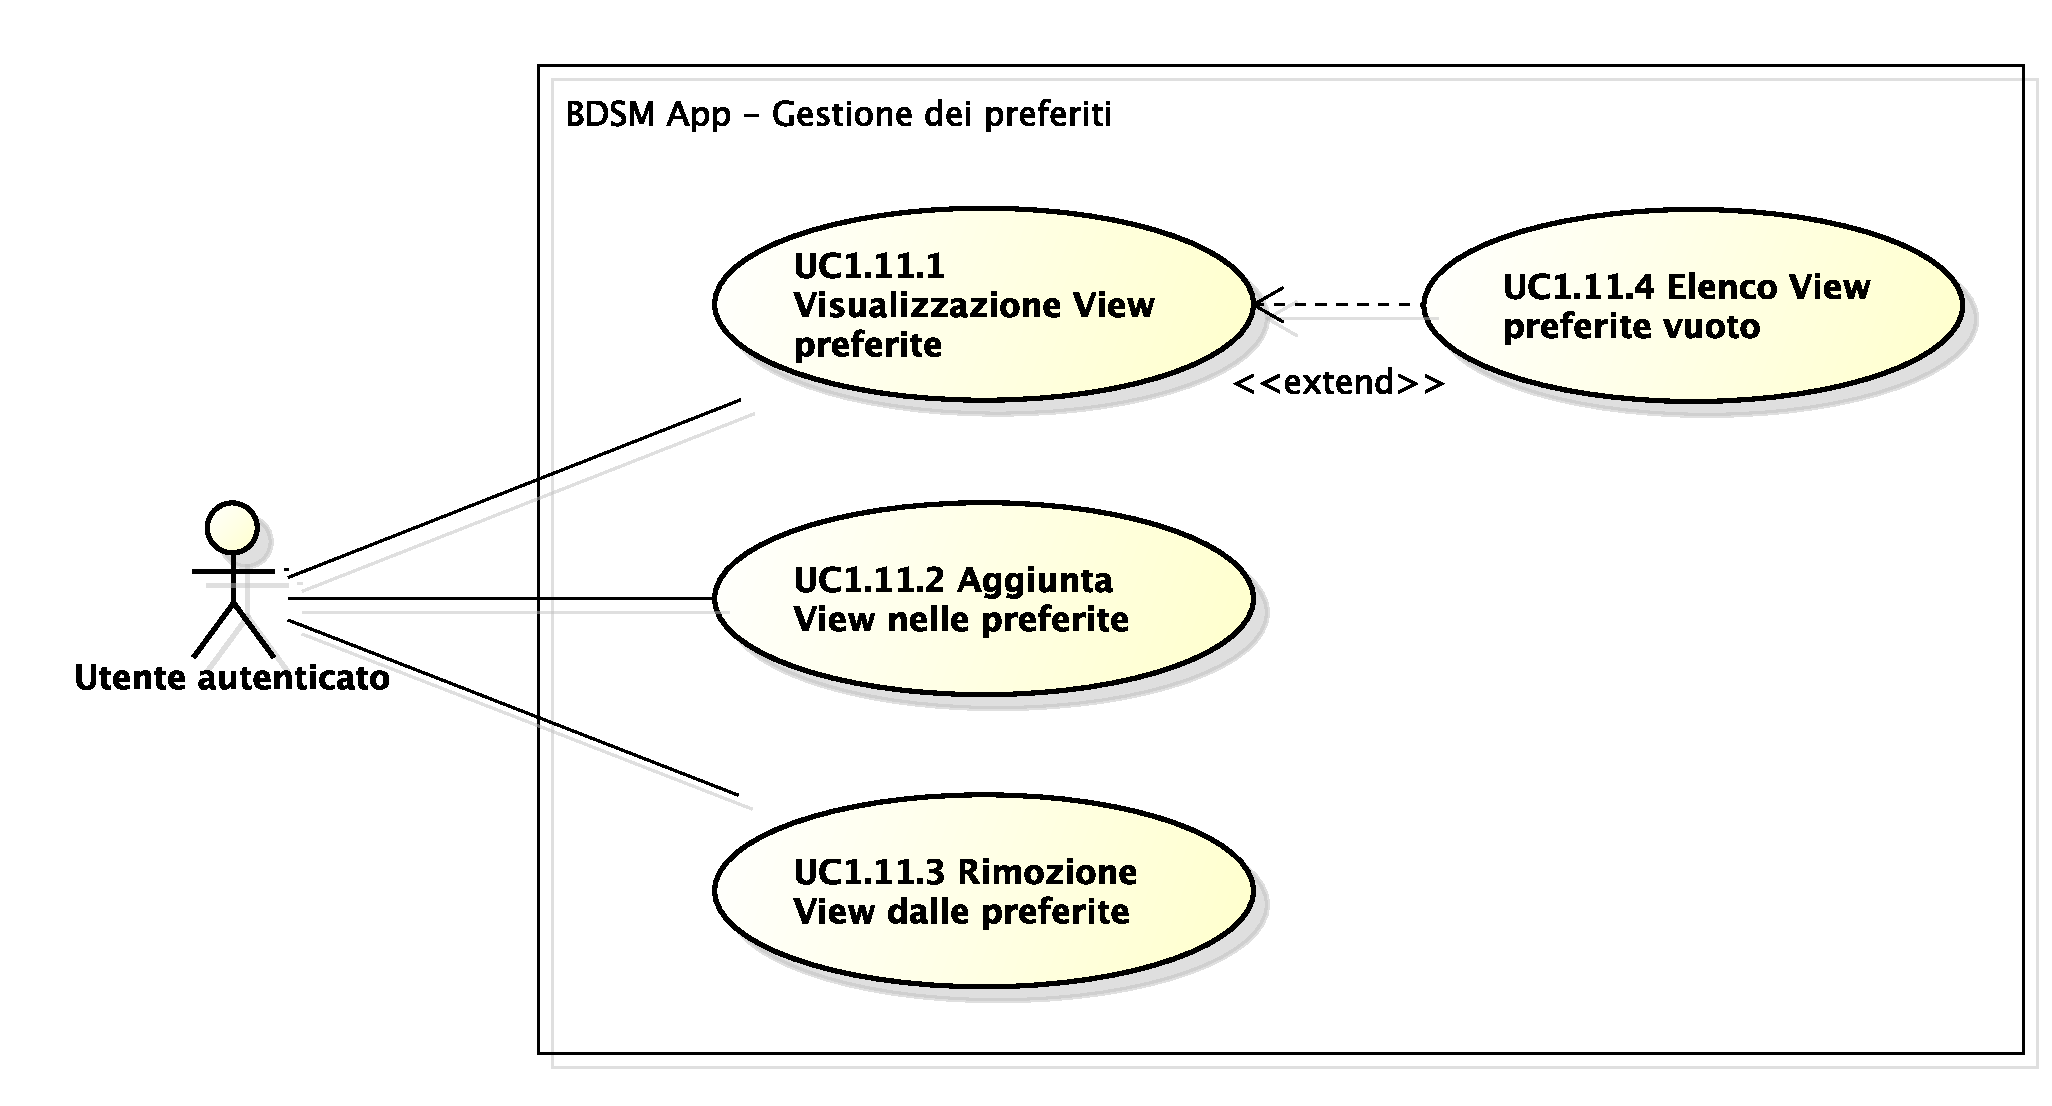
\includegraphics[scale=0.50]{./images/UC1_11.pdf}}
	\caption{UC1.11 - Gestione dei preferiti}
\end{figure}

\begin{itemize}
	\item \textbf{Attori:}
	\begin{itemize}
		\item utente autenticato: utente autenticato che ha accesso al servizio;
	\end{itemize}
	\item \textbf{Descrizione:} gli utenti possono gestire le View che più gli piacciono, in modo da ritrovarle più facilmente e velocemente in caso volessero consultare frequentemente;
	\item \textbf{Precondizione:} l'utente vuole visualizzare le View che ha tra quelle preferite o inserire/rimuovere di nuove/vecchie;
	\item \textbf{Flusso principale degli eventi:}
	\begin{enumerate}
		\item Visualizzazione View preferite (UC1.11.1);
		\item Aggiunta View nelle preferite (UC1.11.2);
		\item Rimozione View dalle preferite (UC1.11.3).
	\end{enumerate}
	\item \textbf{Postcondizione:} l'utente ha visualizzato le View preferite o è andato a aggiungerne di nuove/rimuoverne alcune precedentemente marcate;
	\item \textbf{Estensioni:}
	\begin{itemize}
		\item Elenco View preferite vuoto (UC1.11.4);
	\end{itemize}
\end{itemize}
% FINE USE CASE %

\subsubsection{UC1.11.1: Visualizzazione View preferite}
\begin{itemize}
	\item \textbf{Attori:}
	\begin{itemize}
		\item utente autenticato: utente autenticato che ha accesso al servizio;
	\end{itemize}
	\item \textbf{Descrizione:} l'utente vuole vedere e consultare tutte le View che ha già marcato come preferite;
	\item \textbf{Precondizione:} l'utente deve avere già marcato come preferita qualche View;
	\item \textbf{Scenario principale:} l'utente seleziona l'apposita voce del menù per accedere ai preferiti;
	\item \textbf{Postcondizione:} l'utente visualizza le View marcate come preferite.
\end{itemize}
% FINE USE CASE %

\subsubsection{UC1.11.2: Aggiunta View nelle preferite}
\begin{itemize}
	\item \textbf{Attori:}
	\begin{itemize}
		\item utente autenticato: utente autenticato che ha accesso al servizio;
	\end{itemize}
	\item \textbf{Descrizione:} l'utente desidera marcare una View come preferita. Per farlo deve premere su un apposito pulsante vicino alla View in questione;
	\item \textbf{Precondizione:} l'utente sta visualizzando una o più View nella pagina dedicata;
	\item \textbf{Scenario principale:} l'utente preme sull'apposito pulsante per fare diventare la View una delle preferite;
	\item \textbf{Postcondizione:} l'utente riceve conferma del fatto che la View è entrata a fare parte di quelle preferite.
\end{itemize}
% FINE USE CASE %


\subsubsection{UC1.11.3: Rimozione View dalle preferite}
\begin{itemize}
	\item \textbf{Attori:}
	\begin{itemize}
		\item utente autenticato: utente autenticato che ha accesso al servizio;
	\end{itemize}
	\item \textbf{Descrizione:} l'utente desidera rimuovere una View dalle preferite. Per farlo deve premere su un apposito pulsante vicino alla View in questione;
	\item \textbf{Precondizione:} l'utente visualizza l'elenco delle View aggiunte ai preferiti;
	\item \textbf{Scenario principale:} l'utente preme l'apposito pulsante per rimuovere una View dai preferiti;
	\item \textbf{Postcondizione:} l'utente riceve conferma del fatto che la View è stata rimossa da quelle preferite.
\end{itemize}
% FINE USE CASE %

\subsubsection{UC1.11.4: Elenco View preferite vuoto}
\begin{itemize}
	\item \textbf{Attori:}
	\begin{itemize}
		\item utente autenticato: utente autenticato che ha accesso al servizio;
	\end{itemize}
	\item \textbf{Descrizione:} l'utente visualizza la pagina dei preferiti ma nessuna View risulta marcata come preferita;
	\item \textbf{Precondizione:} l'utente si trova nella pagina dei preferiti e non ha aggiunto nessuna View ai preferiti;
	\item \textbf{Scenario principale:} l'utente visualizza un messaggio il quale lo avverte che nessuna View è stata aggiunta ai preferiti;
	\item \textbf{Postcondizione:} l'utente riceve conferma del fatto che l'elenco delle View aggiunte ai preferiti è vuoto.
\end{itemize}
% FINE USE CASE %

\pagebreak



\subsection{UC2: Servizi REST}
\begin{figure}[htbp]
	\centering
	\centerline{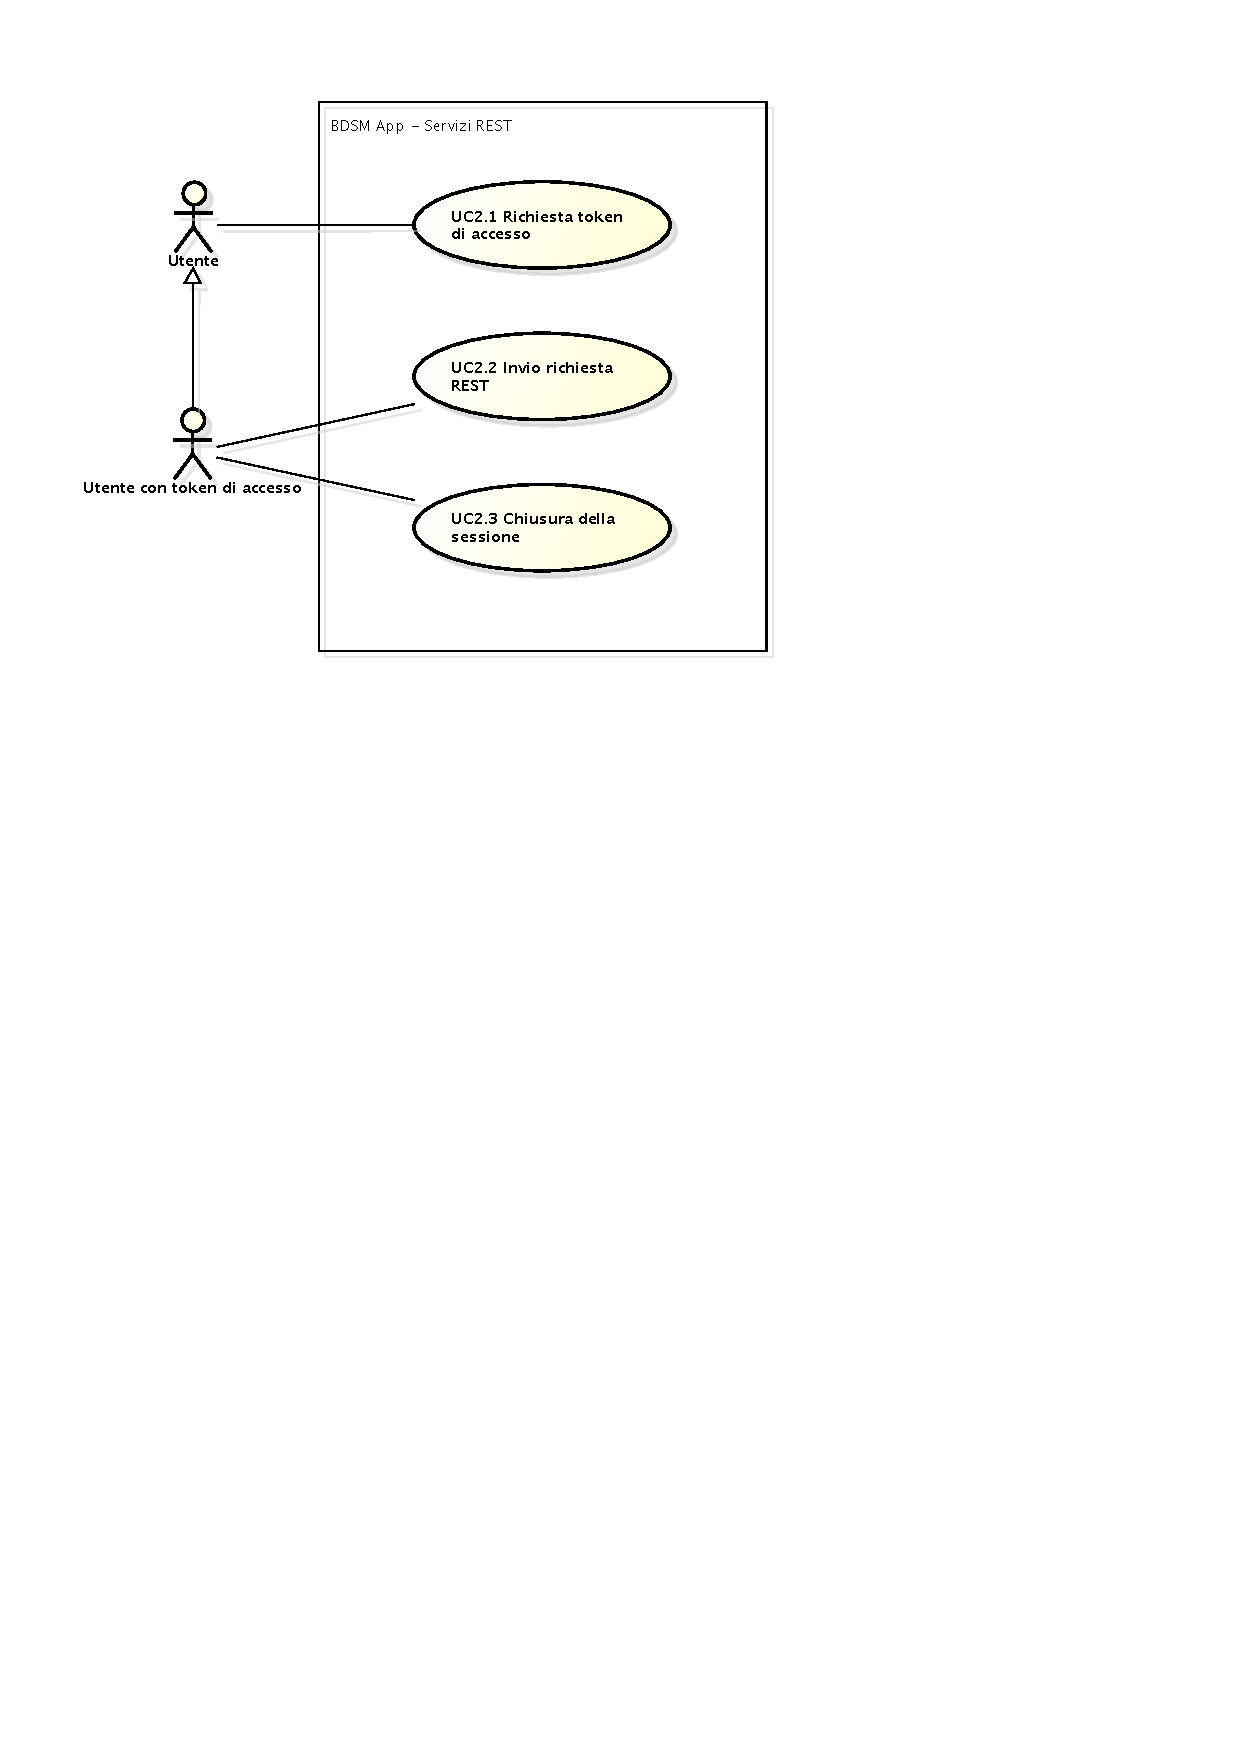
\includegraphics[scale=0.50]{./images/UC2.pdf}}
	\caption{UC2 - Servizi REST}
\end{figure}

\begin{itemize}
	\item \textbf{Attori:}
	\begin{itemize}
		\item utente autenticato: utente che ha effettuato l'accesso nell'applicazione;
		\item utente autenticato con token di accesso: utente che ha ricevuto dal sistema le credenziali (token) per utilizzare i servizi REST offerti;
	\end{itemize}
	\item \textbf{Descrizione:} dopo l'accesso all'applicativo:
	\begin{itemize}
		\item un utente può richiedere un token di accesso premendo su un apposito pulsante;
		\item un utente con token di accesso può fare ciò che può fare l'utente, e in più può inviare una richiesta REST usando il suo token. Può inoltre richiedere che venga rimosso quando non gli è più necessario o se ne desidera ottenere uno nuovo;
	\end{itemize}
	\item \textbf{Precondizione:} l'utente o l'utente con token di accesso dispongono di una connessione con il sistema. Dispongono inoltre di un username e una password riconosciute del sistema ottenute registrandosi tramite l'interfaccia Web.
	\item \textbf{Flusso principale degli eventi:}
	\begin{enumerate}
		\item Richiesta token di accesso (UC2.1);
		\item Invio richiesta REST (UC2.2);
		\item Invalidamento del token di accesso (UC2.3);
		\item Visualizzazione specifica servizi REST (UC2.4);
	\end{enumerate}
	\item \textbf{Postcondizione:} il servizio ha erogato correttamente le funzionalità richieste dall'utente;
\end{itemize}
% FINE USE CASE %

\pagebreak


\subsection{UC2.1: Richiesta token di accesso}
\begin{figure}[htbp]
	\centering
	\centerline{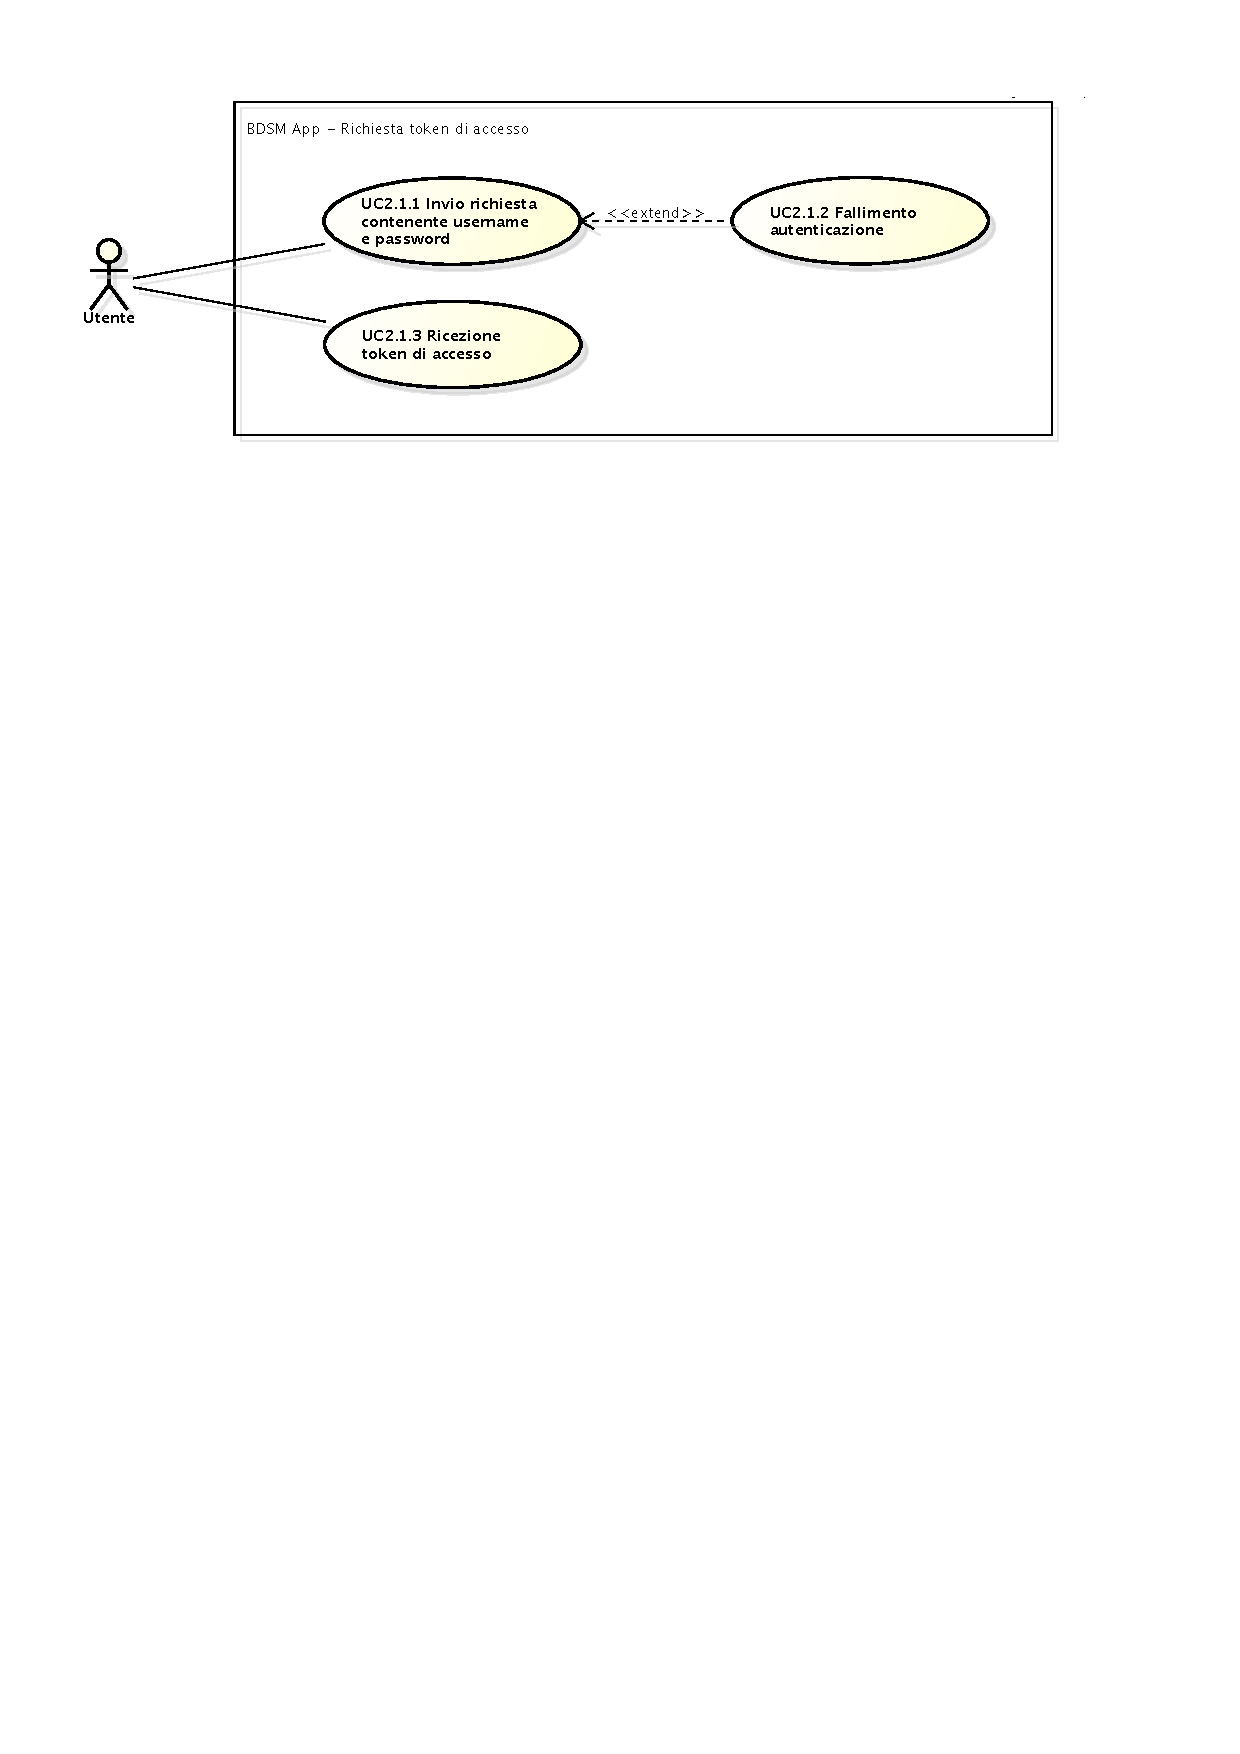
\includegraphics[scale=0.50]{./images/UC2_1.pdf}}
	\caption{UC2.1 - Richiesta token di accesso}
\end{figure}

\begin{itemize}
	\item \textbf{Attori:}
	\begin{itemize}
		\item utente autenticato: utente che desidera ottenere un token di accesso;
	\end{itemize}
	\item \textbf{Descrizione:} l'utente può ottenere un token di accesso per i servizi REST inviando l'apposita richiesta;
	\item \textbf{Precondizione:} l'utente desidera avere un nuovo token di accesso;
	\item \textbf{Flusso principale degli eventi:}
	\begin{enumerate}
		\item Invio richiesta di un token (UC2.1.1);
		\item Ricezione token di accesso (UC2.1.2);
	\end{enumerate}
	\item \textbf{Postcondizione:} l'utente ha ottenuto un token di accesso;
\end{itemize}
% FINE USE CASE %

\subsubsection{UC2.1.1: Invio richiesta di un token}
\begin{itemize}
	\item \textbf{Attori:}
	\begin{itemize}
		\item utente autenticato: utente che desidera ottenere un token di accesso;
	\end{itemize}
	\item \textbf{Descrizione:} l'utente invia la richiesta premendo l'apposito bottone per la generazione di un token;
	\item \textbf{Precondizione:} l'utente si è registrato presso il sistema e non ha ancora associato un token d'accesso oppure ne possiede un token invalidato;
	\item \textbf{Scenario principale:} l'utente preme l'apposito pulsante per effettuare la richiesta di un token d'accesso;
	\item \textbf{Postcondizione:} il sistema riceve la richiesta inviata dall'utente.
\end{itemize}
% FINE USE CASE %

\subsubsection{UC2.1.2: Ricezione token di accesso}
\begin{itemize}
	\item \textbf{Attori:}
	\begin{itemize}
		\item utente autenticato: utente che desidera ottenere un token di accesso;
	\end{itemize}
	\item \textbf{Descrizione:} Il sistema ritorna un token di accesso per l'utente che l'ha richiesto;
	\item \textbf{Precondizione:} il sistema aveva ricevuto una richiesta da un utente registrato per fornire un token di accesso;
	\item \textbf{Scenario principale:} l'utente visualizza il token ricevuto;
	\item \textbf{Postcondizione:} l'utente ha ottenuto un token di accesso valido e lo ha visualizzato.
\end{itemize}
% FINE USE CASE %

\pagebreak


\subsection{UC2.2: Invio richiesta REST}
\begin{figure}[htbp]
	\centering
	\centerline{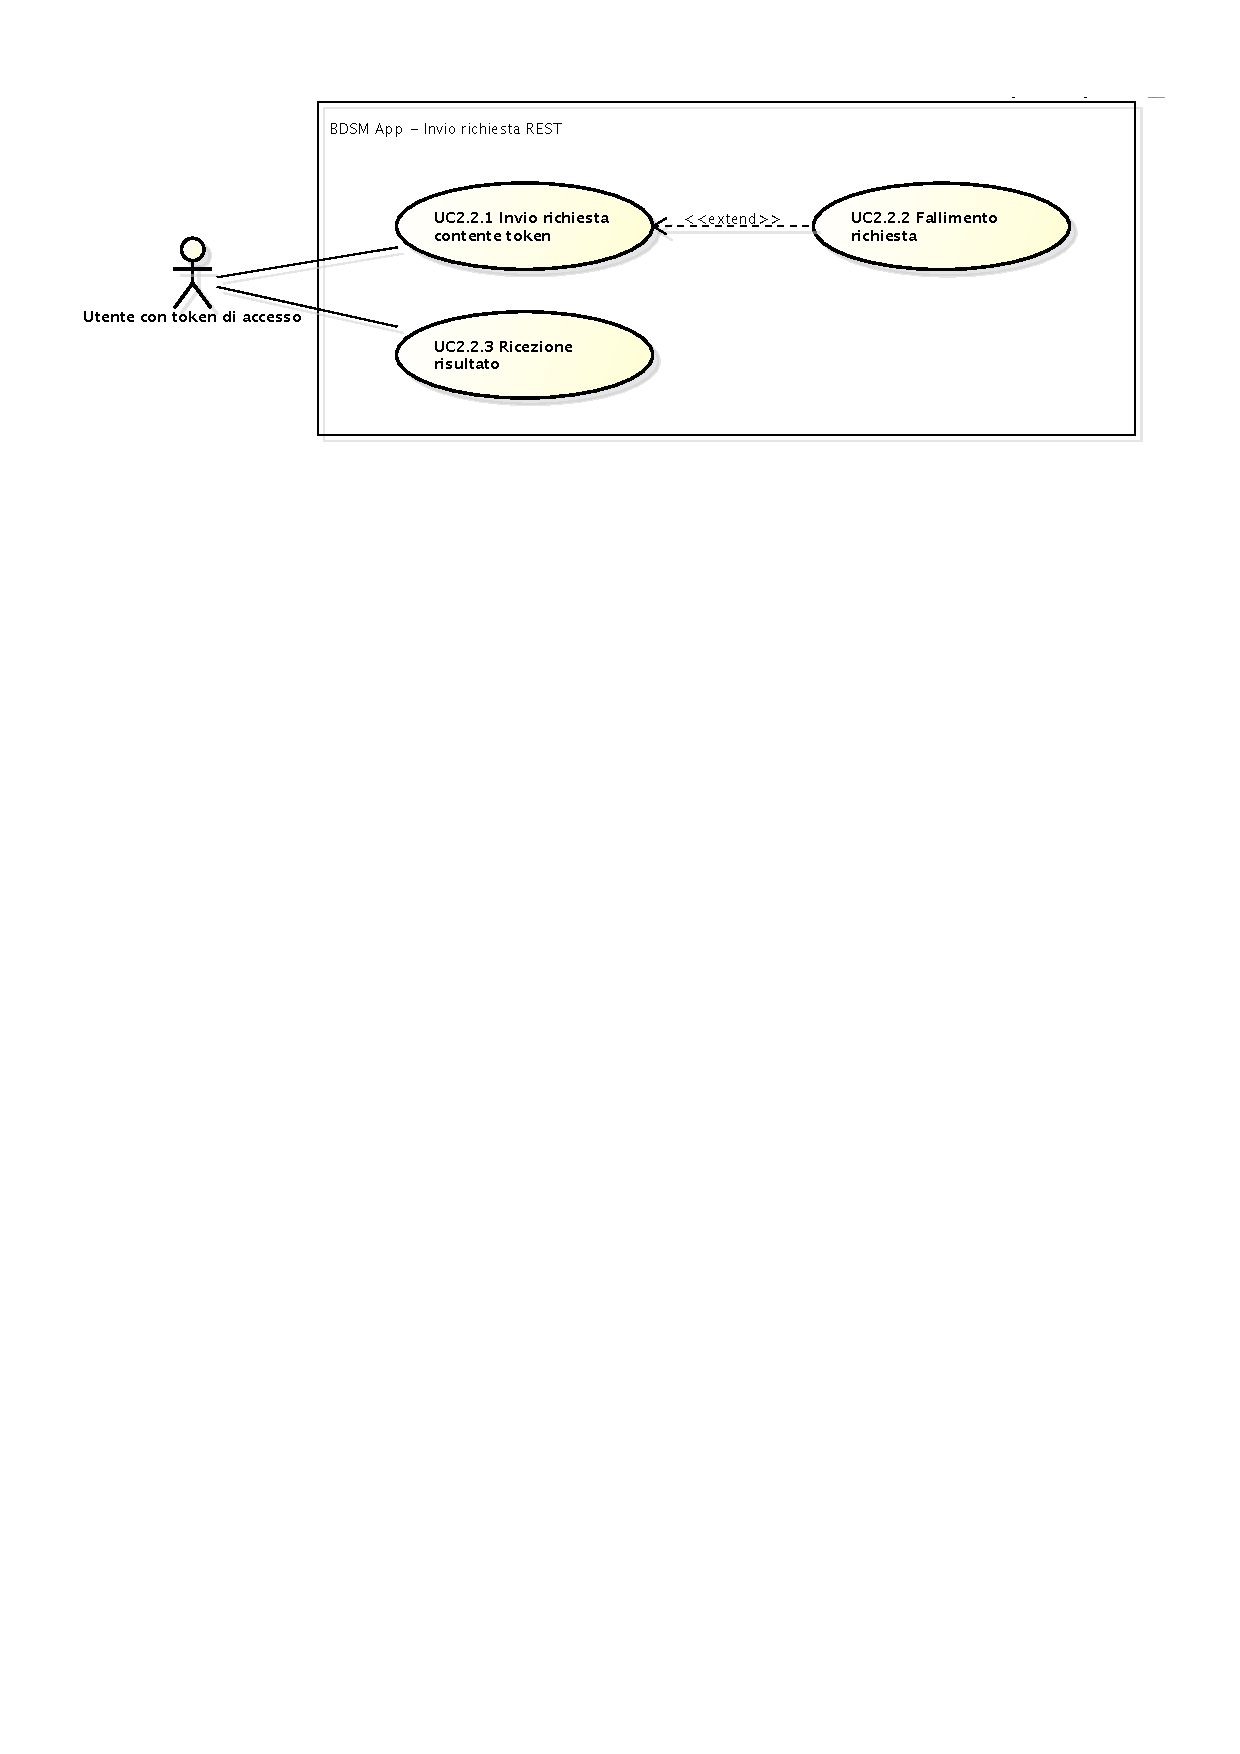
\includegraphics{./images/UC2_2.pdf}}
	\caption{UC2.2 - Invio richiesta REST}
\end{figure}

\begin{itemize}
	\item \textbf{Attori:}
	\begin{itemize}
		\item utente con token di accesso: utente che ha ricevuto dal sistema le credenziali per accedere al servizio;
	\end{itemize}
	\item \textbf{Descrizione:} un utente registrato al sistema può inviare richieste REST al sistema per ottenere i dati di una View senza utilizzare l'interfaccia Web;
	\item \textbf{Precondizione:} l'utente possiede un token di accesso valido;
	\item \textbf{Flusso principale degli eventi:}
	\begin{enumerate}
		\item Invio richiesta contenente token (UC2.2.1);
		\item Ricezione risultato (UC2.2.3);
	\end{enumerate}
	\item \textbf{Postcondizione:} l'utente ha ricevuto i dati richiesti;
	\item \textbf{Estensioni:} Fallimento richiesta (UC2.2.2).
\end{itemize}
% FINE USE CASE %

\subsubsection{UC2.2.1: Invio richiesta contenente token}
\begin{itemize}
	\item \textbf{Attori:}
	\begin{itemize}
		\item utente con Token di accesso: utente che ha ricevuto dal sistema le credenziali per accedere al servizio;
	\end{itemize}
	\item \textbf{Descrizione:} l'utente invia una richiesta avente come parametro il token di accesso;
	\item \textbf{Precondizione:} l'utente possiede un token di accesso valido;
	\item \textbf{Scenario principale:} l'utente effettua la richiesta tramite il token ricevuto;
	\item \textbf{Postcondizione:} il sistema riceve la richiesta inviata.
\end{itemize}
% FINE USE CASE %

\subsubsection{UC2.2.2: Fallimento richiesta}
\begin{itemize}
	\item \textbf{Attori:}
	\begin{itemize}
		\item utente con Token di accesso: utente che ha ricevuto dal sistema le credenziali per accedere al servizio;
	\end{itemize}
	\item \textbf{Descrizione:} il sistema ritorna un errore riportando se il token è non valido o se è stato commesso un errore di sintassi;
	\item \textbf{Precondizione:} l'utente ha inviato una richiesta usando un token non valido o con un errore di sintassi;
	\item \textbf{Scenario principale:} l'utente visualizza un messaggio contenente gli errori riscontrati nella richiesta;
	\item \textbf{Postcondizione:} l'utente ha preso atto del fallimento della richiesta.
\end{itemize}
% FINE USE CASE %

\subsubsection{UC2.2.3: Ricezione risultato}
\begin{itemize}
	\item \textbf{Attori:}
	\begin{itemize}
		\item utente con Token di accesso: utente che ha ricevuto dal sistema le credenziali per accedere al servizio;
	\end{itemize}
	\item \textbf{Descrizione:} vengono ritornati all'utente i dati che aveva richiesto;
	\item \textbf{Precondizione:} l'utente aveva inviato una richiesta corretta al sistema;
	\item \textbf{Scenario principale:} l'utente riceve i dati richiesti;
	\item \textbf{Postcondizione:} l'utente ha ricevuto i dati richiesti.
\end{itemize}
% FINE USE CASE %

\pagebreak


\subsection{UC2.3: Invalidamento del token di accesso}
\begin{figure}[htbp]
	\centering
	\centerline{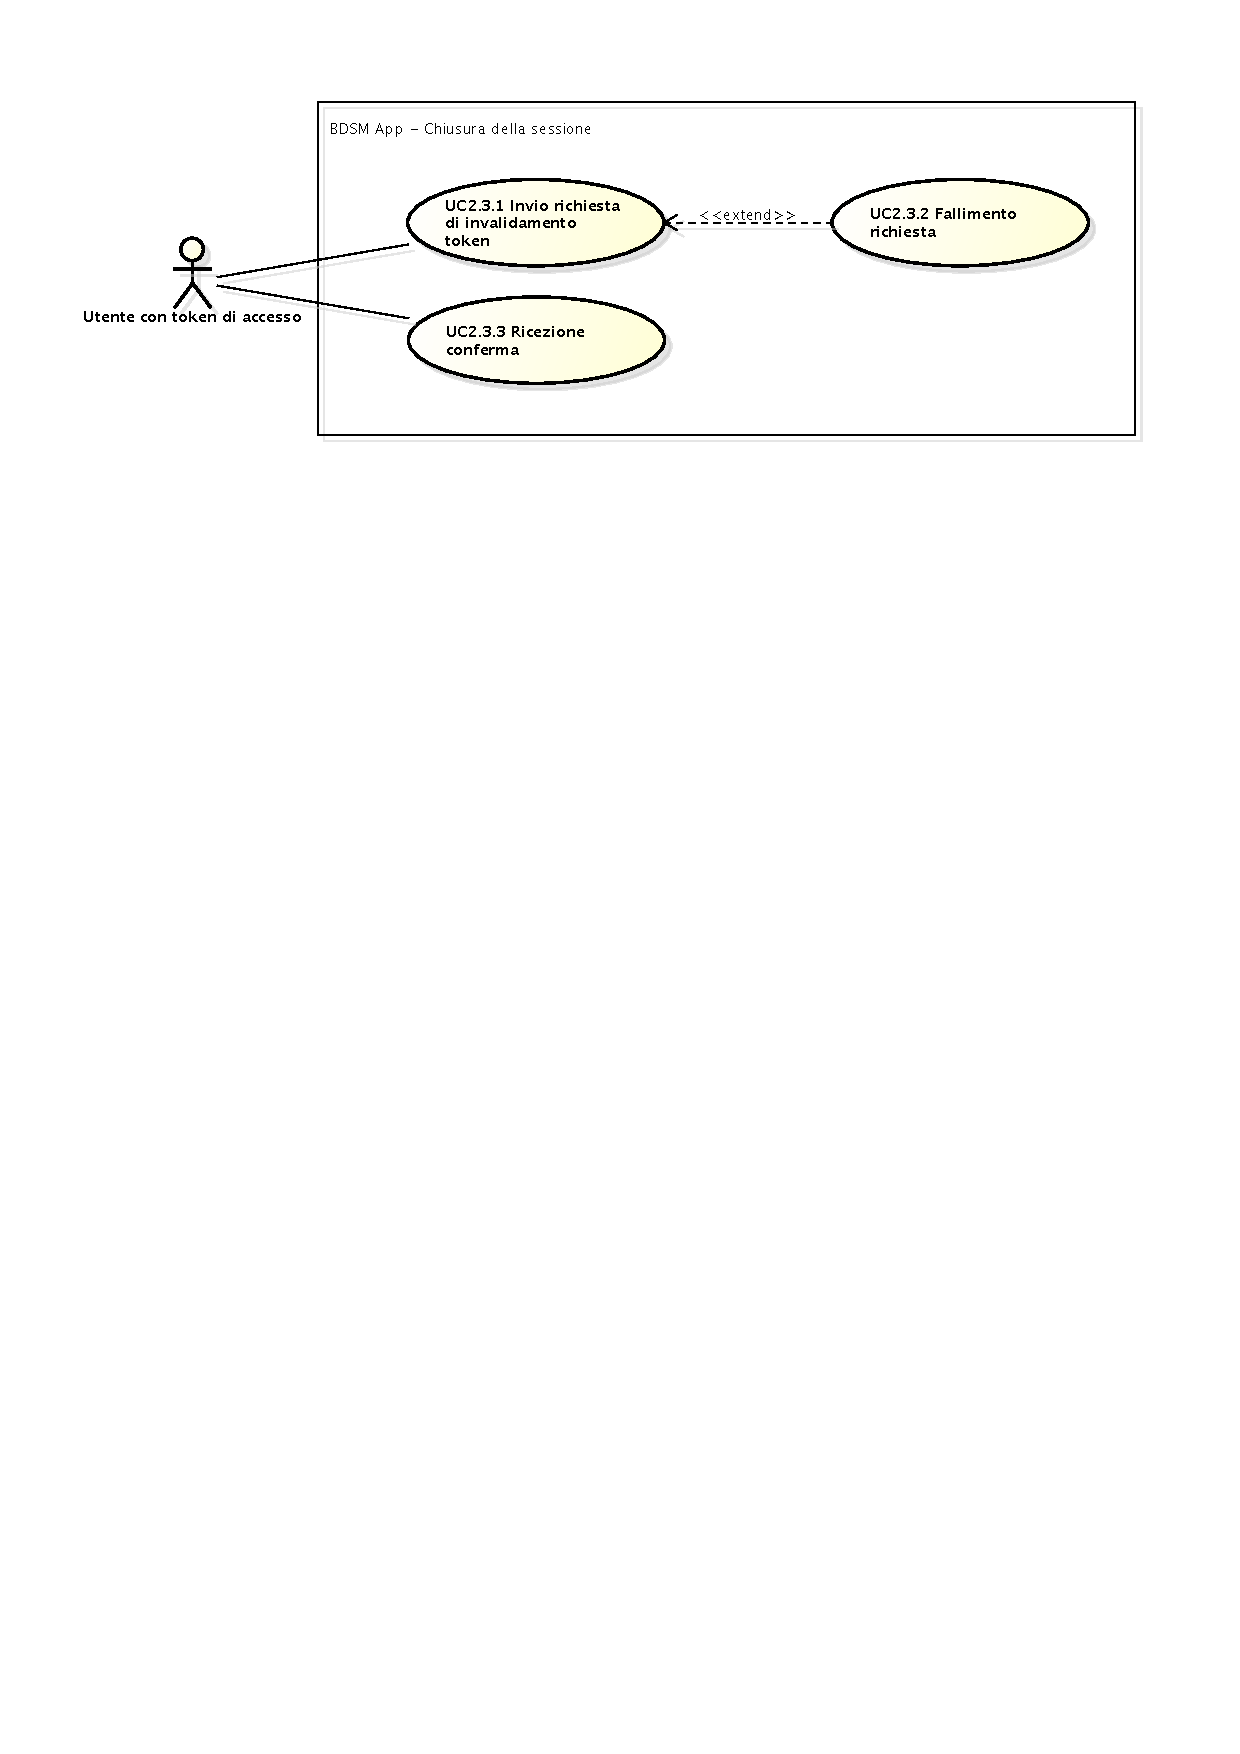
\includegraphics[scale=0.50]{./images/UC2_3.pdf}}
	\caption{UC2.3 - Invalidamento del token di accesso}
\end{figure}

\begin{itemize}
	\item \textbf{Attori:}
	\begin{itemize}
		\item utente con Token di accesso: utente che ha ricevuto dal sistema le credenziali per utilizzare i servizi REST offerti;
	\end{itemize}
	\item \textbf{Descrizione:} l'utente può richiedere che un token di accesso di cui dispone venga disabilitato e dunque non possa essere più usato per accedere ai servizi;
	\item \textbf{Precondizione:} l'utente dispone di un token di accesso valido;
	\item \textbf{Flusso principale degli eventi:}
	\begin{enumerate}
		\item Invio richiesta di invalidamento token (UC2.3.1);
		\item Ricezione conferma (UC2.3.3);
	\end{enumerate}
	\item \textbf{Postcondizione:} il token di accesso non è più valido;
	\item \textbf{Estensioni:} Fallimento richiesta (UC2.3.2).
\end{itemize}
% FINE USE CASE %

\subsubsection{UC2.3.1: Invio richiesta di invalidamento token}

\begin{itemize}
	\item \textbf{Attori:}
	\begin{itemize}
		\item utente con Token di accesso: utente che ha ricevuto dal sistema le credenziali per utilizzare i servizi REST offerti;
	\end{itemize}
	\item \textbf{Descrizione:} l'utente, premendo su un apposito bottone, invia una richiesta che desidera venga disabilitato il token associato al suo account;
	\item \textbf{Precondizione:} il token di cui viene richiesta la disabilitazione è valido;
	\item \textbf{Scenario principale:} l'utente preme l'apposito pulsante per la richiesta di invalidamento del token;
	\item \textbf{Postcondizione:} il token di accesso non è più valido.
\end{itemize}
% FINE USE CASE %

\subsubsection{UC2.3.2: Fallimento richiesta}
\begin{itemize}
	\item \textbf{Attori:}
	\begin{itemize}
		\item utente con Token di accesso: utente che ha ricevuto dal sistema le credenziali per utilizzare i servizi REST offerti;
	\end{itemize}
	\item \textbf{Descrizione:} il sistema avvisa che qualcosa è andato storto durante la disabilitazione del token;
	\item \textbf{Precondizione:} l'utente ha chiesto l'invalidamento di un token;
	\item \textbf{Scenario principale:} l'utente visualizza un messaggio che riporta l'errore riscontrato;
	\item \textbf{Postcondizione:} l'utente ha preso atto del fatto che l'invalidamento del token non ha avuto successo.
\end{itemize}
% FINE USE CASE %

\subsubsection{UC2.3.3: Ricezione conferma}
\begin{itemize}
	\item \textbf{Attori:}
	\begin{itemize}
		\item utente con Token di accesso: utente che ha ricevuto dal sistema le credenziali per utilizzare i servizi REST offerti;
	\end{itemize}
	\item \textbf{Descrizione:} il sistema ritorna una conferma dell'avvenuta invalidazione del token;
	\item \textbf{Precondizione:} l'utente ha chiesto l'invalidamento di un token valido;
	\item \textbf{Scenario principale:} l'utente visualiizza un messaggio che conferma l'invalidamento del token;
	\item \textbf{Postcondizione:} l'utente ha preso atto del fatto che il token è stato invalidato.
\end{itemize}
% FINE USE CASE %

\subsection{UC2.4: Visualizzazione specifica servizi REST}
\begin{itemize}
	\item \textbf{Attori:}
	\begin{itemize}
		\item utente: utente che desidera avere le informazione riguardanti i servizi REST pubblici offerti dal sistema;
	\end{itemize}
	\item \textbf{Descrizione:} l'utente può visualizzare l'elenco dei vari servizi REST offerti dal sistema, in modo da poterli utilizzare a sua volta per scopi personali;
	\item \textbf{Precondizione:} l'utente è autenticato al sistema e si trova nella home page;
	\item \textbf{Scenario principale:} l'utente ha selezionato l'apposita voce che porta alla pagina di visualizzazione dei servizi REST offerti;
	\item \textbf{Postcondizione:} l'utente ha ottenuto l'elenco dei servizi REST offerti.
\end{itemize}
% FINE USE CASE %

\pagebreak
